\chapter{Application-Agnostic Techniques to Reduce Network Transmission}
\label{chapter: bandwidth}

WCAs continuously stream sensor data to the cloudlet. The richer a sensing
modality is, the more information can be extracted. The core sensing modality of
WCAs is visual data, e.g. egocentric images and videos from wearable cameras.
Compared to other sensors, e.g. microphones and inertial measurement units
(IMUs), cameras capture visual information with rich semantics. As commercial
camera hardware becomes more affordable, they become increasingly pervasive in
recent years. For example, in 2013, it is estimated that there are 5.9 million
security cameras in the UK~\cite{Barrett2013}. In the meantime, deep neural
networks (DNNs) have driven significant advancement in computer vision in recent
years and have achieved human-level accuracy in many previously untractable
perception problems (e.g. face recognition, image
classification)~\cite{learned2016labeled, schroff2015facenet}. The richness and
the open-endness of visual data makes camera the ideal sensor for WCAs.

However, continuous video transmission from many Tier-3 devices places severe
stress on the wireless spectrum.  Hulu estimates that its video streams require
13 Mbps for 4K resolution and 6 Mbps for HD resolution using highly optimized
offline encoding~\cite{Hulu2017}. Live streaming is less bandwidth-efficient, as
confirmed by our measured bandwidth of 10 Mbps for HD feed at 25 FPS. Just 50
users transmitting HD video streams continuously can saturate the theoretical
uplink capacity of 500 Mbps in a 4G LTE cell that covers a large rural
area~\cite{LteWorld2009}.  This is clearly not scalable.

In this chapter, we show how per-user bandwidth demand in WCA-like live video
analytics can be significantly reduced using an application-agnostic approach.
We aim to reduce bandwidth demand without compromising the timeliness or
accuracy of results. We present techniques for an adaptive computer vision
pipeline for Tier-3 devices that leverages edge computing to enable dynamic
optimizations. In contrast to previous
works~\cite{Wang2017networked}~\cite{zhang2015design}~\cite{Wang2016skyeyes}, we
leverage state-of-the-art deep neural networks (DNNs) to selectively transmit
interesting data from a video stream and explore environment-specific
optimizations. 

This chapter is organized as follows. We first discuss the challenges of running
DNNs for visual perception solely on Tier-3 devices in
Section~\ref{bw:challenges}. Next, we propose and compare two
application-agnostic techniques to reduce network transmission in edge computing
context. We present our results first in the context of live video analytics for
small autonomous drones. Both as emerging Tier-3 devices, drones and wearable
devices face similar challenges in live video analysis. Finally, we showcase how
these techniques can be applied to WCAs in Section~\ref{bw:wca}.

\section{Video Processing on Mobile Devices}
\label{bw:challenges}

In the context of real-time video analytics, Tier-3 devices represent
fundamental mobile computing challenges that were identified two decades
ago~\cite{Satya1996}.  Two challenges have specific relevance here. First,
mobile elements are resource-poor relative to static elements.  Second, mobile
connectivity is highly variable in performance and reliability.  We discuss
their implications below.


\subsection{Computation Power on Tier-3 Devices}
\label{bw:payload}

Unfortunately, the hardware needed for deep video stream processing in real time
is larger and heavier than what can fit on a typical Tier-3 device. State-of-art
techniques in image processing use DNNs that are compute- and memory-intensive.
Figure~\ref{fig:onboard-dnn-speed} presents experimental results on two
fundamental computer vision tasks, image classification and object detection, on
four different devices. In the figure, MobileNet V1 and ResNet101 V1 are image
classification DNNs. Others are object detection DNNs. We use publicly available
pretrained DNN models for measurements~\cite{tfod2019}. We carefully choose
hardware platforms to represent a range of computation capabilities of Tier-3
devices. To anticipate future improvements in smartphone technology, our
experiments also consider more powerful devices such as the
Intel$^{\tiny\textregistered}$ Joule~\cite{Hardawar2016} and the NVIDIA
Jetson~\cite{NVIDIA2017} that are physically compact and light enough to be
credible as wearable device platforms in the future.

Note that the absolute speed of DNN inference depends on a wide range of
factors, including the optimizations used in DNN model implementation, the
choice of linear algebra libraries, the presence of vectorized instructions and
hardware accelerators. In Fig.~\ref{fig:onboard-dnn-speed}, we present the best
results we could obtain on each platform. This is not intended to directly
compare frameworks and platforms (as others have been
doing~\cite{Zhang2018pcamp}), but rather to illustrate the differences between
wearable platforms and fixed infrastructure servers. 

\begin{figure}
\centering
\begin{flushleft}
M: MobileNet V1; R: ResNet101 V1;
S-M: SSD MobileNet V1; S-I: SSD Inception V2;\\F-I: Faster R-CNN Inception V2;
F-R: Faster R-CNN ResNet101 V1
\end{flushleft}
\sisetup{
    table-format=3,
    table-number-alignment=left
}
\hspace{-0.8in}
\begin{tabular}{|p{1.3cm}|S[table-column-width=1.3cm]|p{3.0cm}|p{1.8cm}|S[table-column-width=1.2cm]|S[table-column-width=1.4cm]|S[table-column-width=1.3cm]|S[table-column-width=1.3cm]|S[table-format=4, table-number-alignment=left, table-column-width=1.5cm]|S[table-format=5, table-number-alignment=left, table-column-width=1.9cm]|}
\hline
{\multirow{2}{*}{}} & {\multirow{2}{*}{}} & {\multirow{2}{*}{}}                                        & {\multirow{2}{*}{}}                                                                        & \multicolumn{2}{c|}{\parbox[t]{1.8cm}{\centering Image\\Classification\\~}}                                & \multicolumn{4}{c|}{Object Detection} \\ \cline{5-10}
                  &  {\parbox[t]{0.9cm}{\centering Weight\\(g)}}
                  & \centering CPU
                  & \centering GPU
                  & {\parbox[t]{0.9cm}{\centering M\\(ms)}}
                  & {\parbox[t]{1.1cm}{\centering R\\(ms)}}
                  & {\parbox[t]{1.0cm}{\centering S-M\\(ms)}}
                  & {\parbox[t]{1.0cm}{\centering S-I\\(ms)}}
                  & {\parbox[t]{1.3cm}{\centering F-I\\(ms)}}
                  & {\parbox[t]{1.6cm}{\centering F-R\\(ms)}} \\ \hline
Nexus~6    & 184                                                      & 4-core 2.7 GHZ Krait 450, 3GB Mem                           & Adreno 420                                                                              & 353 {\scriptsize \ (67)}                                                 & 983 {\footnotesize \ (141)}                                                   & 441 {\footnotesize \ (60)           }                               & 794 {\footnotesize \ (44)            }                                       & {\small ENOMEM}                                                                 & {\small ENOMEM}                                                               \\ \hline
Intel$^{\tiny \textregistered}$ Joule 570x     & 25                                                       & 4-core 1.7 GHz Intel Atom$^{\tiny\textregistered}$ T5700, 4GB Mem                          & Intel$^{\tiny\textregistered}$ HD Graphics (gen 9)                                                               & 37 {\scriptsize \ (1)$\ddagger$ }                                       & 183 {\footnotesize \ (2)$\dagger$$\ddagger$ }                                        & 73  {\footnotesize \ (2)$\ddagger$ }                               & 442 {\footnotesize \ (29)            }                                       & 5125 {\footnotesize \ (750)}                                                             & 9810 {\footnotesize \ (1100)}                                                          \\ \hline
NVIDIA Jetson TX2     & 85                                                       & 2-Core 2.0 GHz Denver2 + 4-Core 2.0 GHz Cortex-A57, 8GB Mem & 256 cuda core 1.3 GHz NVIDIA Pascal                                                          & 13 {\scriptsize \ (0)$\dagger$  }                                       & 92 {\footnotesize \ (2)$\dagger$ }                                          & 192 {\footnotesize \ (18)           }                               & 285 {\footnotesize \ (7)$\dagger$   }                                       & {\small ENOMEM}                                                                 & {\small ENOMEM}                                                               \\ \hline
Rack-mounted Server     &                                                          & 2x 36-core 2.3 GHz Intel$^{\tiny\textregistered}$ Xeon$^{\tiny\textregistered}$ E5-2699v3 Processors, 128GB Mem     & 2880 cuda core 875MHz NVIDIA Tesla K40, 12GB GPU Mem                             & 4 {\scriptsize \ (0)$\ddagger$  }                                       & 33 {\footnotesize \ (0)$\dagger$  }                                          & 12  {\footnotesize \ (2)$\ddagger$ }                               & 70  {\footnotesize \ (6)             }                                       & 229 {\footnotesize \ (4)$\dagger$}                                                               & 438 {\footnotesize \ (5)$\dagger$}                                                               \\ \hline
\end{tabular}
\begin{captiontext}
\vspace{0.1in}
Figures above are means of 3 runs across 100 random images. The time shown
includes only the forward pass time using batch size of 1. ENOMEM indicates
failure due to insufficient memory. Figures in parentheses are standard
deviations. The weight figures for Joule and Jetson include only the modules
without breakout boards. Weight for Nexus~6 includes the complete phone with
battery and screen. Numbers are obtained with TensorFlow (TensorFlow Lite for
Nexus 6) unless indicated otherwise. \\
$\dagger$ indicates GPU is used. $\ddagger$ indicates
Intel$^{\tiny\textregistered}$ Computer Vision SDK beta 3 is used.
\end{captiontext}
\caption{Deep Neural Network Inference Speed on Tier-3 Devices}
\label{fig:onboard-dnn-speed}
\end{figure}

Image classification is a computer vision task that maps an image into
categories, with each category indicating whether one or many particular objects
(e.g., a human survivor, a specific animal, or a car) exist in the image. Two
widely used multiclass classificaiton DNNs are tested. Their prediction speed
are shown in column ``Image Classification''. One of the DNNs, MobileNet
V1~\cite{Howard2017}, is designed for mobile devices from the ground-up by
reducing the number of parameters and simplifying the layer computation using
depth-wise separable convolution. On the other hadn, ResNet101 V1~\cite{He2016}
is a more accurate but also more resource-hungry DNN that won the highly
recognized ImageNet classification challenge in 2015~\cite{Russakovsky15}. 

Also shown is another harder computer vision task, object detection. Object
detection is a more difficult perception problem, because it not only requires
categorization, but also prediction of bounding boxes around the specific areas
of an image that contains a object. Object detection DNNs
are built on top of image classification DNNs by using image classification DNNs
as low-level feature extractors. Since feature extractors in object detection
DNNs can be changed, the DNN structures excluding feature detectors are referred
as object detection meta-architectures. We benchmarked two object detection DNN
meta-architectures: Single Shot Multibox Detector (SSD)~\cite{Liu2016} and
Faster R-CNN~\cite{Ren2015}. We used multiple feature extractors for each
meta-architecture. The meta-architecture SSD uses simpler methods to identify
potential regions for objects and therefore requires less computation and runs
faster. On the other hand, Faster R-CNN~\cite{Ren2015} uses a separate region
proposal neural network to predict regions of interest and has been shown to
achieve higher accuracy~\cite{Huang2017} for difficult tasks.
Figure~\ref{fig:onboard-dnn-speed} presents results in four columns: SSD
combined with MobileNet V1 or Inception V2, and Faster R-CNN combined with
Inception V2 or ResNet101 V1~\cite{He2016}. The combination of Faster R-CNN and
ResNet101 V1 is one of the most accurate object detectors available
today~\cite{Russakovsky15}. The entries marked ``{\sc ENOMEM}'' correspond to
experiments that were aborted because of insufficient memory.

These results demonstrates the computation gap between mobile and static
elements. While the most accurate object detection model Faster R-CNN Resnet101
V1 can achieve more than two FPS on a server GPU, it either takes several
seconds on Tier-3 devices or fails to execute due to insufficient memory. In
addition, the figure also confirms that sustaining open-ended real-time video
analytics on smartphone form factor computing devices is well beyond the state
of the art today and may remain so in the near future.  This constrains what is
achievable with Tier-3 devices alone.

\subsection{Result Latency, Offloading \& Scalability}
\label{bw:offloading}

{\em Result latency} is the delay between first capture of a video frame in
which a particular result is present, and report of its discovery or feedback
based on the discovery after video processing. Operating totally disconnected, a
Tier-3 device can capture and store video, but defer its processing until the
mission is complete.  At that point, the data can be uploaded from the device to
the cloud and processed there.  This approach completely eliminates the need for
real-time video processing, obviating the challenges of Tier-3 computation power
mentioned previously. Unfortunately, this approach delays the discovery and use
of knowledge in the captured data by a substantial amount (e.g., many tens of
minutes to a few hours).  Such delay may be unacceptable in use cases such as
search-and-rescue using drones, or real-time step-by-step instruction feedback
in WCAs. In this chapter, we focus on approaches that aim for much smaller,
real-time result latency.

A different approach is to offload video processing in real-time over a wireless
link to an edge computing node. With this approach, even a weak Tier-3 device
can leverage the substantial processing capability of a ground-located cloudlet,
without concern for its weight, size, heat dissipation or energy usage.  Much
lower result latency is now possible.  However even if cloudlet resources are
viewed as ``free'' from the viewpoint of mobile computing, the Tier-3 device
consumes wireless bandwidth in transmitting video.

Today, 4G LTE offers the most plausible wide-area connectivity from a Tier-3
device to its associated cloudlet. The much higher bandwidths of 5G are still
several years away, especially at global scale.  More specialized wireless
technologies, such as Lightbridge 2~\cite{LightBridge2} for drones, could also
be used. Regardless of specific wireless technology, the principles and
techniques described in this chapter apply.

When offloading, scalability in terms of maximum number of concurrently
operating Tier-3 devices within a 4G LTE cell becomes an important metric.  In
this chapter, we explore how the limited processing capability on a Tier-3 device
can be used to greatly decrease the volume of data transmitted, thus improving
scalability while minimally impacting result accuracy and result latency.

Note that the uplink capacity of 500 Mbps per 4G LTE cell assumes standard
cellular infrastructure that is undamaged.  In natural disasters and military
combat, this infrastructure may be destroyed. Emergency substitute
infrastructure, such as Google and AT\&T's partnership on balloon-based 4G LTE
infrastructure for Puerto Rico after hurricane Maria~\cite{Morse2017}, can only
sustain much lower uplink bandwidth per cell, e.g. 10Mbps for the balloon-based
LTE~\cite{Sankaran2018}.  Conserving wireless bandwidth from Tier-3 video
transmission then becomes even more important, and the techniques described here
will be even more valuable.

% Another metric of importance here is result accuracy, which influences a
% second dimension of scalability, namely the ability of one individual to
% supervise the result streams from many drones.  The output of each video
% processing pipeline should only demand occasional human attention.  The
% accuracy, sophistication, and speed of this pipeline determines the cognitive
% load on mission personnel for a given video stream.  For example, a pipeline
% that has virtually no false positives or false negatives in detecting survivors
% will consume less supervisory human attention than a mediocre pipeline.  That
% will allow one person to confidently supervise a large swarm that rapidly covers
% a large search area.

\section{Baseline: Dumb  S\lc{trategy}}
\label{sec:dumbdrone}

\subsection{Description}

We first establish and evaluate the baseline case of no image processing
performed at the Tier-3 device.  Instead, all captured video is immediately
transmitted to the cloudlet.  Result latency is very low, merely the sum of
transmission delay and cloudlet processing delay. We use drones as the example
of Tier-3 devices and drone video search as the scenario of video analytics
first. We later demonstrate how to apply the techniques developed to WCAs.

\begin{table}
\centering
\begin{tabular}{|p{1cm}|p{2.5cm}|p{2.5cm}|p{2.5cm}|p{2.5cm}|p{2.5cm}|}
\hline
   & Detection & Data & Data & Training & Testing \\ 
Task& Goal & Source & Attributes & Subset & Subset\\ 
\hline
T1 & {\small People in scenes of daily life}&{\small Okutama Action Dataset~\cite{Barekatain2017}}&\makecell[tl]{\small 33 videos \\\small 59842 fr\\\small 4K@30~fps}&\makecell[tl]{\small 9 videos\\\small 17763 fr}&\makecell[tl]{\small 6 videos\\\small 20751 fr}\\ 
\hline
T2 &{\small Moving cars}&{\small Stanford Drone Dataset~\cite{Robicquet2016}}&\makecell[tl]{\small 60 videos \\\small 522497 fr\\\small 1080p@30~fps}&\makecell[tl]{\small 16 videos\\\small 179992 fr} & \multirow{4}{*}{\parbox{1.5cm}{\centering\small 14 videos 92378 fr\\ Combination of test videos from each dataset.}} \\ \cline{1-5}
  %% \makecell[tl]{\small 14 videos\\\small 92378 fr\\\small Combination of \\\small human, car, raft \\\small and elephant videos\\\small from each datasets}} \\ \cline{1-5}
%% \makecell[tl]{\small 14 videos\\\small 92378 fr}\\ 
%% \hline
T3 &{\small Raft in flooding scene}&{\small YouTube collection~\cite{YouTube1}}&\makecell[tl]{\small 11 videos \\\small 54395 fr\\\small 720p@25~fps}&\makecell[tl]{\small 8 videos\\\small 43017 fr} & \\ \cline{1-5}
%% \makecell[tl]{\small 14 videos\\\small 92378 fr}\\
%% \hline
T4 &{\small Elephants in natural habitat}&{\small YouTube collection~\cite{YouTube2}}&\makecell[tl]{\small 11 videos \\\small 54203 fr\\\small 720p@25~fps}&\makecell[tl]{\small 8 videos\\\small 39466 fr} & \\ \cline{1-5}
%% \makecell[tl]{\small 14 videos\\\small 92378 fr}\\
%% \hline
% T5 &{\small Pushing or pulling Suitcases}&\small Okutama Action Dataset &\small Same as T1 &\small Same as T1 & \\
%% \small Same as T1\\
\hline
\end{tabular}
\vspace{0.1in}
\begin{captiontext}
fr = ``frames''\\
fps = ``frames per second''\\
No overlap between training and testing subsets of data
\end{captiontext}
\caption{Benchmark Suite of Drone Video Traces}
\label{fig:benchmarksuite}
\end{table}

\begin{table}
\centering
\begin{tabular}{|c|c|c|c|c|}
\hline
     & Total & Avg & & \\ 
     & Bytes & BW & & \\ 
Task & (MB) & (Mbps) & Recall & Precision \\ 

\hline
T1 & \phantom{0}924 & 10.7 & 74\% & 92\%\\ 
\hline
T2 & 2704 & \phantom{0}7.0 & 66\% & 90\%\\ 
\hline
\end{tabular}
\vspace{0.2in}
\begin{captiontext}
Peak bandwidth demand is same as average since video is transmitted
continuously. Precision and recall are at the maximum F1 score.
\end{captiontext}
\caption{Baseline Object Detection Metrics}
\label{fig:baseline}
\end{table}

\subsection{Experimental Setup}
\label{sec:dumbdrone-setup}

To ensure experimental reproducibility, our evaluation is based on
replay of a benchmark suite of pre-captured videos rather than on
measurements from live drone flights.  In practice, live results may
diverge slightly from trace replay because of non-reproducible
phenomena.  These can arise, for example, from wireless propagation
effects caused by varying weather conditions, or by seasonal changes
in the environment such as the presence or absence of leaves on trees.
In addition, variability can arise in a  drone's pre-programmed flight
path due to collision avoidance with moving obstacles such as birds,
other drones, or aircraft.

All of the pre-captured videos in the benchmark suite are publicly accessible,
and have been captured from aerial viewpoints. They characterize drone-relevant
scenarios such as surveillance, search-and-rescue, and wildlife conservation.
Table~\ref{fig:benchmarksuite} presents this benchmark suite of videos,
organized into four tasks. All the tasks involve detection of tiny objects on
individual frames. Although T2 is also nominally about action detection (moving
cars), it is implemented using object detection on individual frames and then
comparing the pixel coordinates of vehicles in successive frames.
% Task T5 additionally involves action detection, which operates on short video segments rather than individual frames. 

\subsection{Evaluation}
\label{sec:dumbdrone-results}

Table~\ref{fig:baseline} presents the key performance indicators on the object
detection tasks T1 and T2. We use the well-labeled dataset to train and evaluate
Faster-RCNN with ResNet 101. We report the precision and recall at maximum F1
score.  Peak bandwidth is not shown since it is identical to average bandwidth
demand for continuous video transmission.  As shown earlier in
Table~\ref{fig:onboard-dnn-speed}, the accuracy of this algorithm comes at the
price of very high resource demand.  This can only be met today by server-class
hardware that is available in a cloudlet.  Even on a cloudlet, the figure of 438
milliseconds of processing time per frame indicates that only a rate of two
frames per second is achievable.  Sustaining a higher frame rate will require
striping the frames across cloudlet resources, thereby increasing resource
demand considerably.  Note that the results in
Table~\ref{fig:onboard-dnn-speed} were based on 1080p frames, while tasks T1
uses the higher resolution of 4K. This will further increase demand on cloudlet
resources.

Clearly, the strategy of blindly shipping all video to the cloudlet and
processing every frame is resource-intensive to the point of being impractical
today.  It may be acceptable as an offline processing approach in the cloud, but
is unrealistic for real-time processing on cloudlets.  We therefore explore an
approach in which a modest amount of computation on the Tier-3 is able, with
high confidence, to avoid transmitting many video frames and thereby saving
wireless bandwidth as well as cloudlet processing resources.  This leads us to
the EarlyDiscard strategy of the next section.




\section{{\xc EarlyDiscard} S\lc{trategy}}
\label{sec:earlydiscard}

\subsection{Description}
EarlyDiscard is based on the idea of using on-board processing to filter and
transmit only interesting frames in order to save bandwidth when offloading
computation. Previous work~\cite{Hu2015}~\cite{Naderiparizi2017} leveraged
pixel-level features and multiple sensing modalities to select interesting
frames from hand-held or body-worn cameras. In this work, we explore the use
of DNNs to filter frames from aerial views. The benefits of using DNNs are
twofold. First, DNNs are trained and specialized for each task, resulting in
their high accuracy and robustness. Second, no additional hardware is added to
existing drone platforms.

Although smartphone-class hardware is incapable of supporting the
most accurate object detection algorithms at full frame rate today, it is
typically powerful enough to support less accurate algorithms.  These {\em weak
detectors} are typically designed for mobile platforms or were the state of the
art just a few years ago.  In addition, they can be biased towards high recall
with only modest loss of precision.  In other words, many clearly irrelevant
frames can be discarded by a weak detector, without unacceptably increasing the
number of relevant frames that are erroneously discarded.  This asymmetry is the
basis of the early discard strategy.

As shown in Figure~\ref{fig:ondrone}, we envision a choice of weak detectors
being available as early discard filters on a drone, with the specific choice of
filter being mission-specific.  Relative to the measurements presented in
Figure~\ref{fig:onboard-dnn-speed}, early discard only requires image
classification: it is not necessary to know exactly where in the frame a
relevant object occurs.  This suggests that MobileNet would be a good choice as
a weak detector. Its speed of 13 ms per frame on Jetson yields more than 75 fps.
We therefore use MobileNet on the drone for early discard in our experiments.

Pre-trained classifiers for MobileNet are available today for objects such as
cars, animals, human faces, human bodies, watercraft, and so on.  However, these
DNN classifiers have typically been trained on images that were captured from a
human perspective --- often by a camera held or worn by a person.  A drone,
however, has an aerial viewpoint and objects look rather different.  To improve
classification accuracy on drones, we used {\em transfer learning}~\cite{Yosinski2014} to finetune
the pre-trained classifiers on small training sets of images that were captured
from an aerial viewpoint.  This involves initial re-training of the last DNN
layer, followed by re-training of the entire network until convergence. Transfer
learning enables accuracy to be improved significantly for aerial images without
incurring the full cost of creating a large training set captured from an aerial
viewpoint.

Drone images are typically captured from a significant height, and hence objects
in such an image are small.  This interacts negatively with the design of many
DNNs, which first transform an input image to a fixed low resolution --- for
example, 224x224 pixels in MobileNet. Many important but small objects in the
original image become less recognizable.  It has been shown that small object
size correlates with poor accuracy in DNNs~\cite{Huang2017}.  To address this
problem, we {\em tile} high resolution frames into multiple sub-frames and then
perform recognition on the sub-frames.  This is done offline for training, as
shown in Figure~\ref{fig:tiling}, and also for online inference on the drone and
on the cloudlet.  The lowering of resolution of a sub-frame by a DNN is less
harmful, since the scaling factor is smaller.  Objects are represented by many
more pixels in a transformed sub-frame than if the entire frame had been
transformed.  The price paid for tiling is increased computational demand.  For
example, tiling a frame into four sub-frames results in four times the
classification workload.

\begin{figure}
  \hspace{-0.1in}
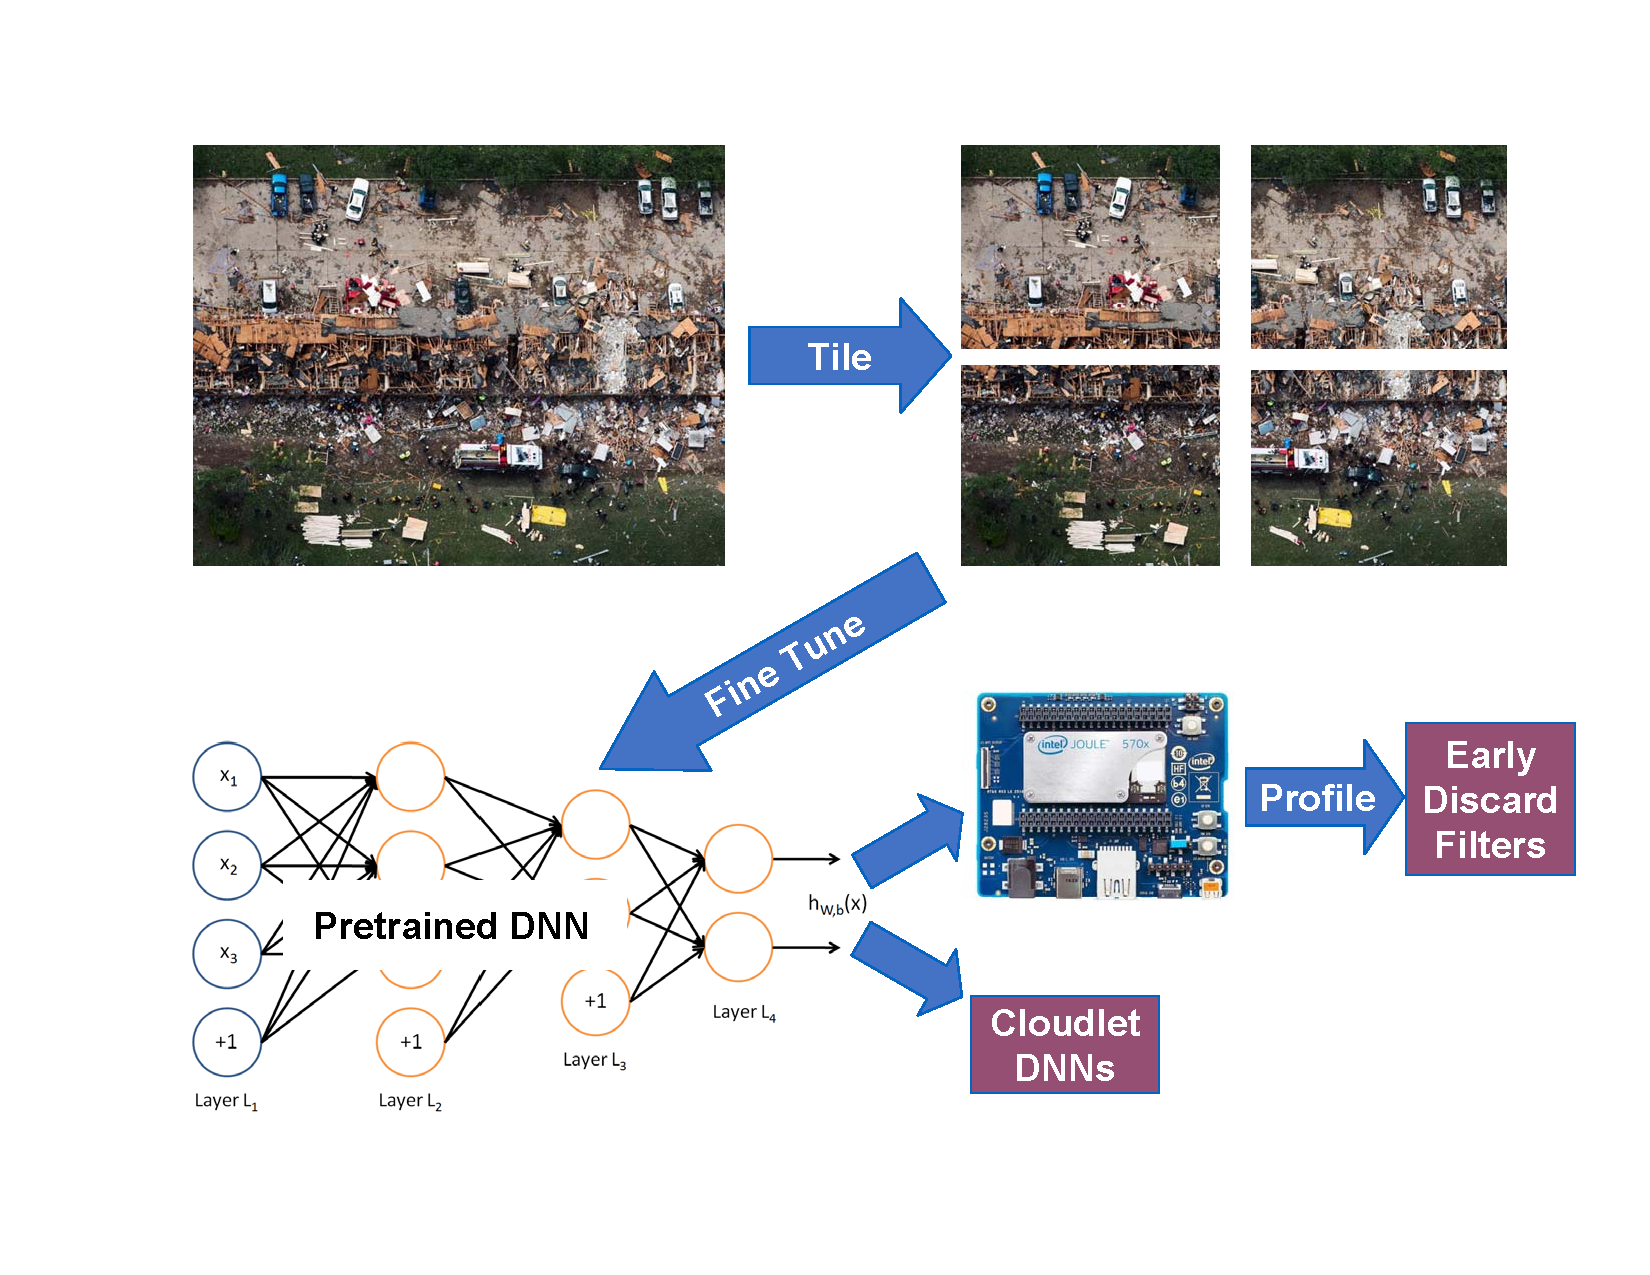
\psfig{file=FIGS/fig-training.pdf, scale=0.35}\\
\caption{Tiling and DNN Fine Tuning}
\label{fig:tiling}
\end{figure}

\subsection{Experimental Setup}

Our experiments on the {\xc EarlyDiscard}
strategy used the same benchmark suite described in
Section~\ref{sec:dumbdrone-setup}. We used Jetson TX2 as the drone platform. We use
both frame-based and event-based metrics to evaluate the MobileNet filters.

\subsection{Results of Early Discard Filters}
\label{sec:earlydiscard-result}

EarlyDiscard is able to significantly reduce the bandwidth consumed while
maintaining high result accuracy and low average delay. For three out of four
tasks, the average bandwidth is reduced by a factor of ten. Below we present
our results in detail.

\begin{figure}
\centering
\hspace*{-0.3in}
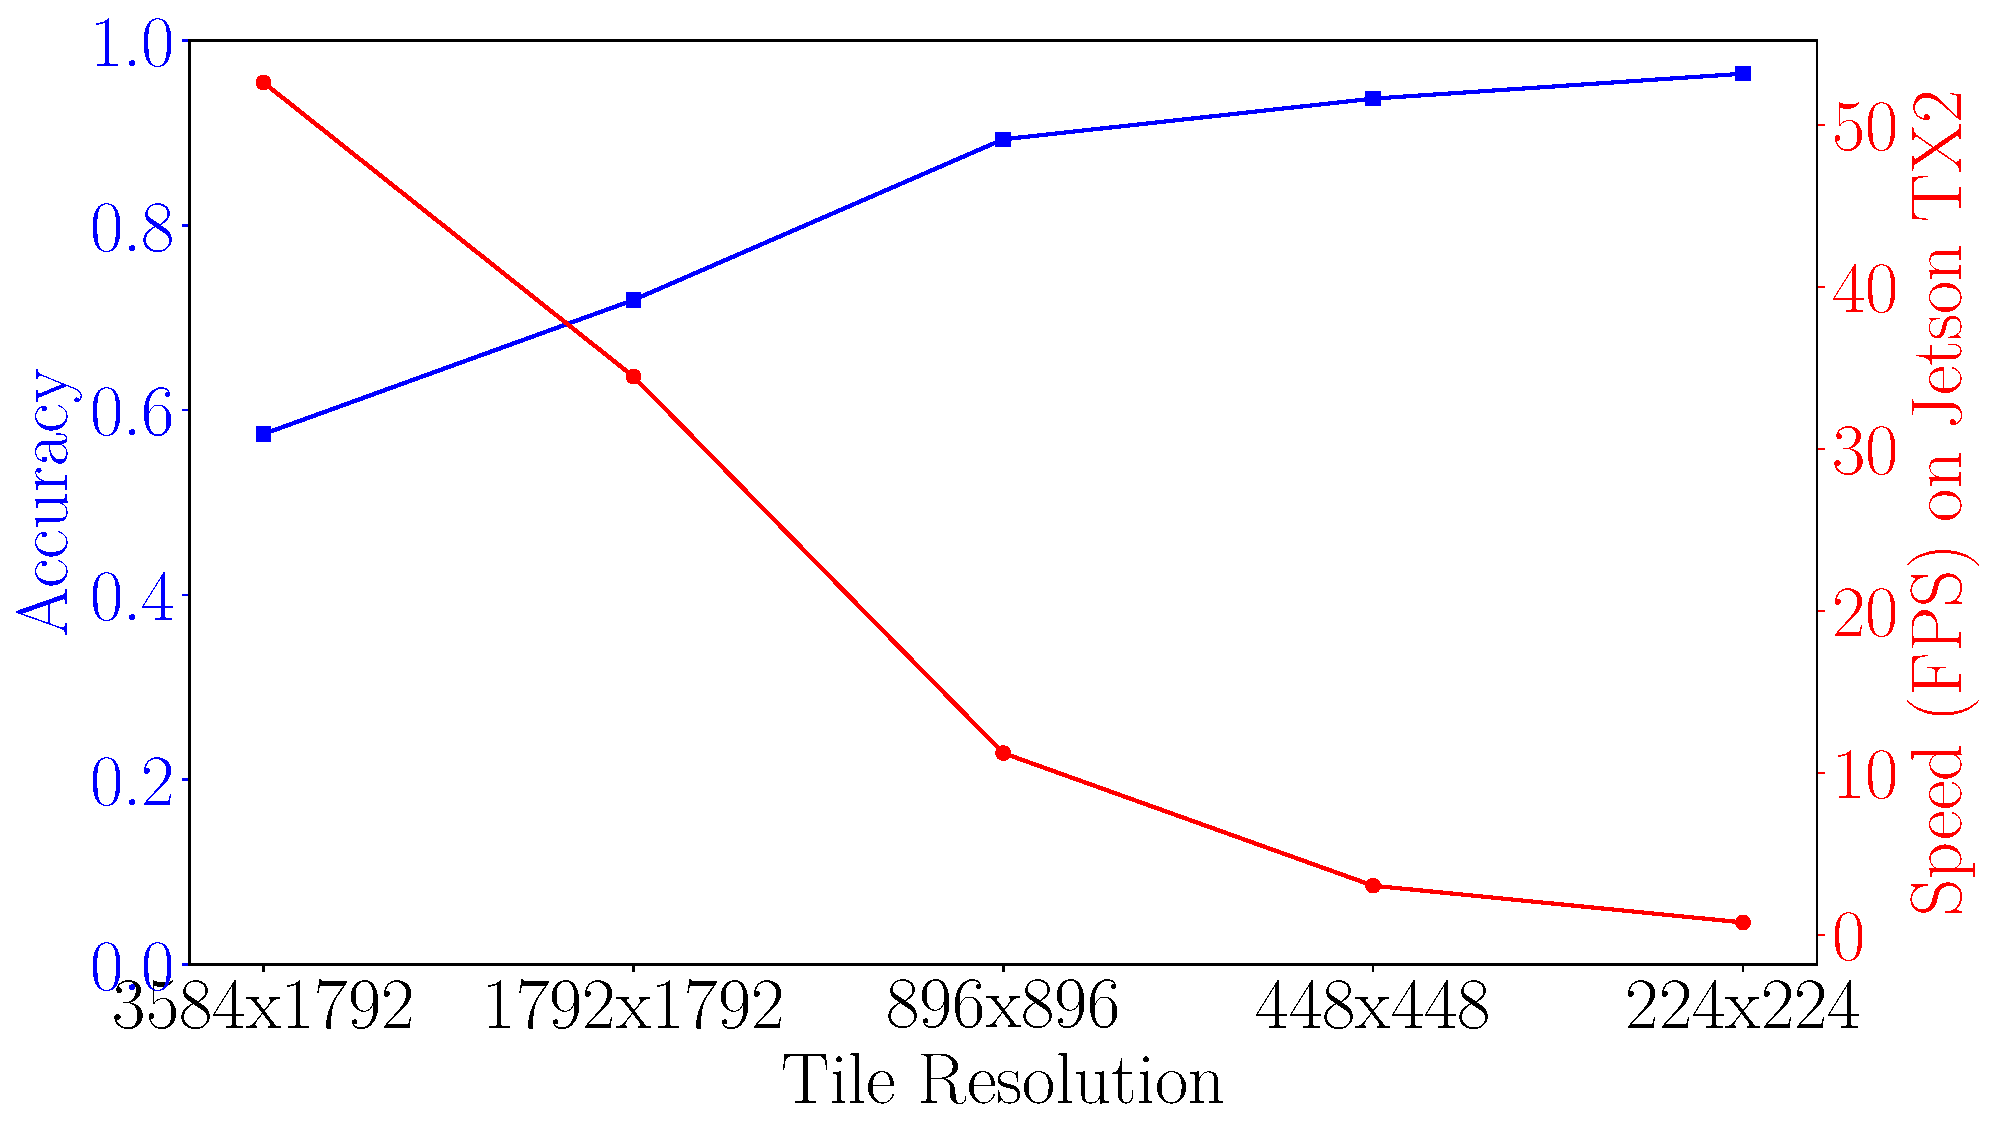
\psfig{file=FIGS/fig-tile-resolution-speed-accuracy.pdf, scale=0.2}
\caption{Speed-Accuracy Trade-off of Tiling}
\label{fig:earlydiscard-tile-accuracy-speed}
\vspace{-0.1in}
\end{figure}


\noindent{\textbf{Effects of Tiling}}: Tiling is used to improve the accuracy
for high resolution aerial images. We used the Okutama Action Dataset, whose
attributes are shown in row T1 of Figure~\ref{fig:benchmarksuite}, to explore
the effects of tiling.  For this dataset,
Figure~\ref{fig:earlydiscard-tile-accuracy-speed} shows how speed and accuracy
change with tile size.  Accuracy improves as tiles become smaller, but the
sustainable frame rate drops.  We group all tiles from the same frame in a
single batch to leverage parallelism, so the processing does not change linearly
with the number of tiles. The choice of an operating point will need to strike a
balance between the speed and accuracy.  In the rest of the paper, we use two
tiles per frame by default. 

\noindent{\textbf{Drone Filter Accuracy}}: The output of a drone filter is the
probability of the current tile being ``interesting.''  A tunable {\em cutoff
threshold} parameter specifies the threshold for transmission to the cloudlet.
All tiles, whether deemed interesting or not, are still stored in the drone
storage for post-mission processing.

Figure~\ref{fig:earlydiscard-frame-percent-breakdown} shows our results on all
four tasks. Events such as detection of a raft in T3 occur in consecutive
frames, all of which contain the object of interest. A correct detection of an
event is defined as at least one of the consecutive frames being transmitted to
the cloudlet.  Blue lines in
Figure~\ref{fig:earlydiscard-frame-percent-breakdown} shows how the event
recalls of drone filters for different tasks change as a function of cutoff
threshold. The MobileNet DNN filter we used is able to detect all the events for
T1 and T4 even at a high cutoff threshold. For T2 and T3, the majority of the
events are detected. Achieving high recall on T2 and T3 (on the order of 0.95 or
better) requires setting a low cutoff threshold.  This leads to the possibility
that many of the transmitted frames are actually uninteresting (i.e., false
positives).

%% \begin{figure}
%% \includegraphics[width=0.6\linewidth]{FIGS/fig-event-recall-vs-threshold.pdf}
%% \vspace{-0.1in}
%% \caption{Drone Filter Recall vs. Cutoff Threshold}
%% \label{fig:event-recall-vs-threshold}
%% \end{figure}


\noindent{\textbf{False negatives}}: As discussed earlier, false negatives are
a source of concern with early discard.  Once the drone drops a frame
containing an important event, improved cloudlet processing cannot help. The
results in the third column of Figure~\ref{fig:early-discard-results} confirm
that there are no false negatives for T1 and T4 at a cutoff threshold of 0.5.
For T2 and T3, lower cutoff thresholds are needed to achieve perfect recalls.

\begin{figure}
    \centering
    
\includegraphics[width=0.8\linewidth]{FIGS/fig-event-recall-frame-percentage-legend.pdf}
    \hspace*{-0.3in}
    \begin{subfigure}[T1]{
        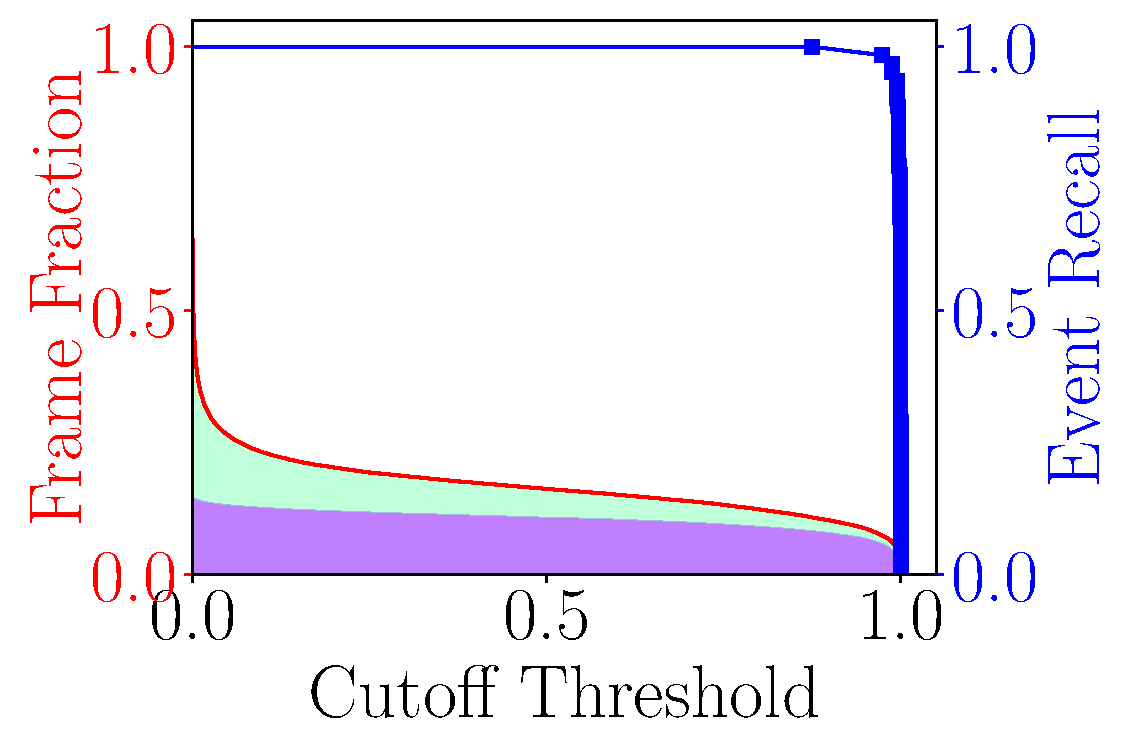
\includegraphics[width=0.5\linewidth]{FIGS/fig-event-recall-frame-percentage-vs-threshold-okutama.pdf}}        
    \end{subfigure}
    \begin{subfigure}[T2]{
      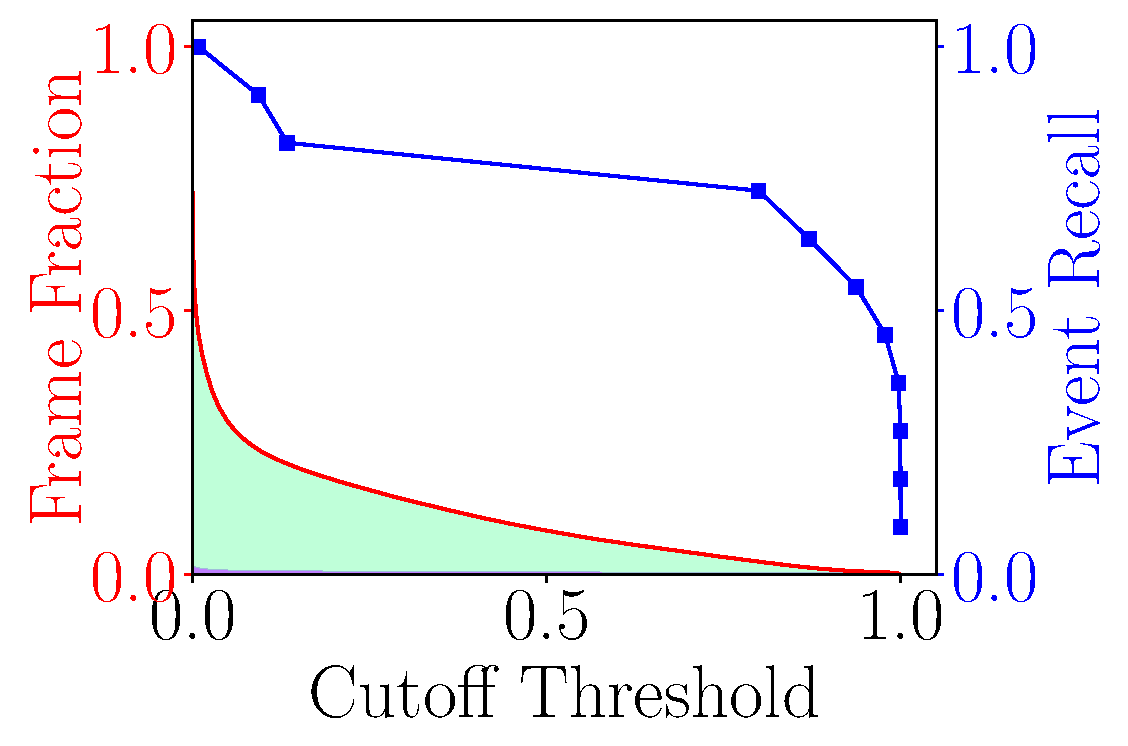
\includegraphics[width=0.5\linewidth]{FIGS/fig-event-recall-frame-percentage-vs-threshold-stanford.pdf}}
    \end{subfigure}
    \hspace*{-0.3in}    
    \begin{subfigure}[T3]{
      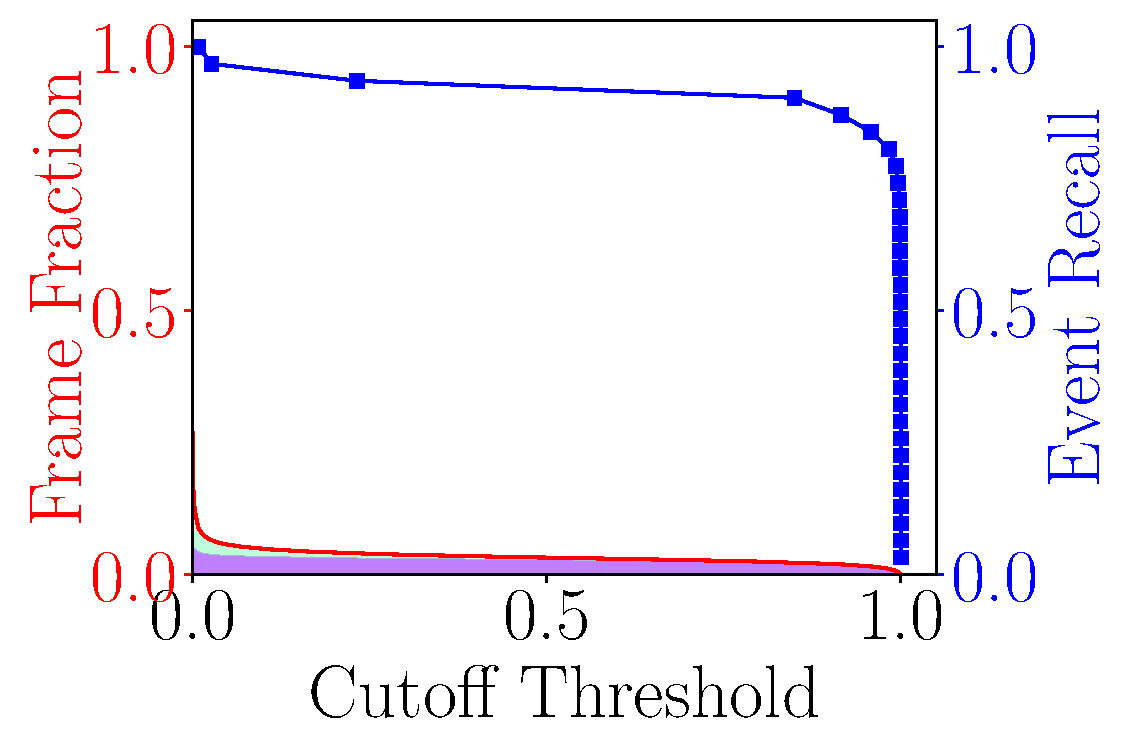
\includegraphics[width=0.5\linewidth]{FIGS/fig-event-recall-frame-percentage-vs-threshold-raft.pdf}}
    \end{subfigure}
    \begin{subfigure}[T4]{
      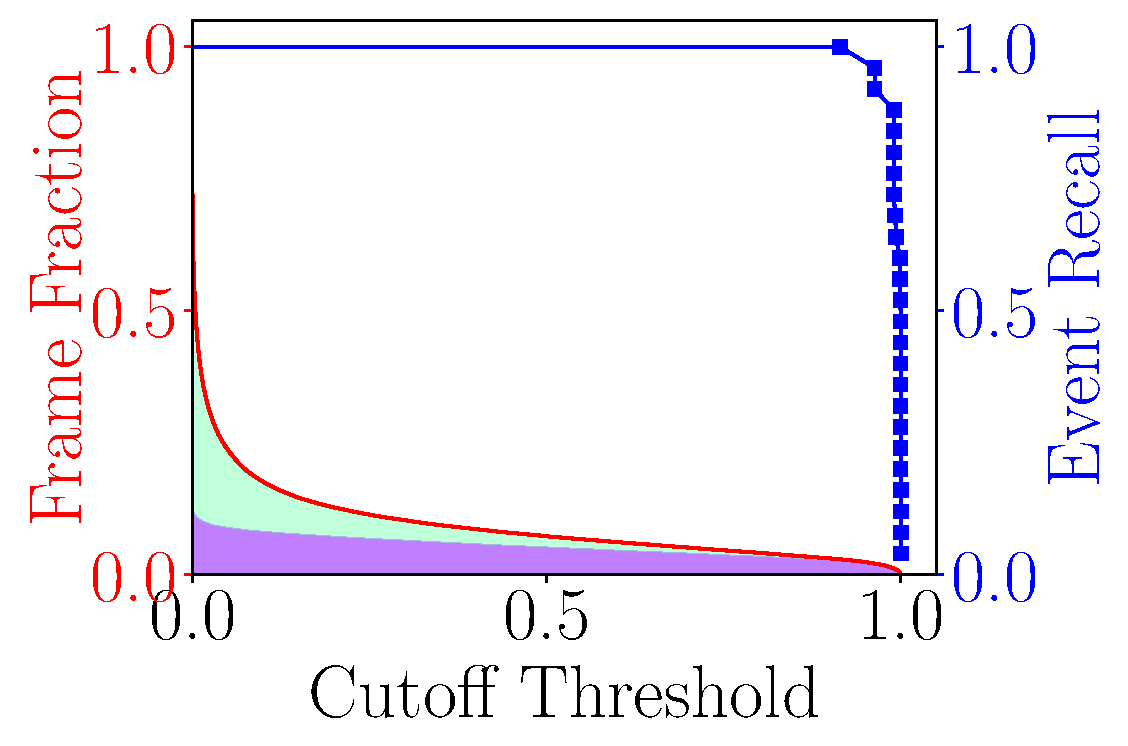
\includegraphics[width=0.5\linewidth]{FIGS/fig-event-recall-frame-percentage-vs-threshold-elephant.pdf}}
    \end{subfigure}
\caption{Where the Bandwidth Goes}
\label{fig:earlydiscard-frame-percent-breakdown}
\end{figure}

\begin{figure}
\hspace{-0.15in}
%\centering
\begin{tabular}{|c|c|c|c|c|c|c|}
\hline
   &Task   &Dete-       &Avg&Total&Avg&Peak\\
   &Total&cted&Delay&Data&B/W&B/W\\
   &Events&Events&(s)&(MB)&(Mbps)&(Mbps)\\ 

\hline
T1 & \phantom{0}62  & 100~\%       &  \phantom{0}0.1&\phantom{0}441  &  5.10     &   10.7  \\
\hline
T2 & \phantom{0}11  & \phantom{0}73~\%      & \phantom{0}4.9 & \phantom{00}13            &  0.03 & \phantom{0}7.0 \\ % 100% recall at 47% of frames, 82% recall at 21% of frames
\hline
T3 & \phantom{0}31  & \phantom{0}90~\%  & 12.7 & \phantom{00}93  &  0.24 &  \phantom{0}7.0 \\ % 100% recall at 9% frames
\hline
T4 & \phantom{0}25  & 100~\%       & \phantom{0}0.3 & \phantom{0}167  &  0.43 &  \phantom{0}7.0 \\
\hline
\end{tabular}\\
\caption{Recall, Event Latency and Bandwidth at Cutoff Threshold 0.5}
\label{fig:early-discard-results}
\end{figure}

\noindent{\textbf{Result latency}}:
The contribution of early discard processing to total result latency
is calculated as the average time difference between the first frame
in which an object occurs (i.e., first occurrence in ground truth) and
the first frame containing the object that is transmitted to the
backend (i.e., first detection).  The results in the fourth column of
Figure~\ref{fig:early-discard-results} confirm that early discard
contributes little to result latency.  The amounts range from 0.1~s
for T1 to 12.7~s for T3.  At the timescale of human actions
such as dispatching of a rescue team, these are negligible delays.

\noindent{\textbf{Bandwidth}}: Columns 5--7 of
Figure~\ref{fig:early-discard-results} pertain to wireless bandwidth demand for
the benchmark suite with early discard.  The figures shown are based on H.264
encoding of each individual frames in the drone-cloudlet video transmission.
Average bandwidth is calculated as the total data transmitted divided by
mission duration.  Comparing column 5 of Figure~\ref{fig:early-discard-results}
with column 2 of Figure~\ref{fig:baseline}, we see that all videos in the
benchmark suite are benefited by early discard (Note T3 and T4 have the same
test dataset as T2). For T2, T3, and T4, the bandwidth is reduced by more than
10x. The amount of benefit is greatest for rare events (T2 and T3).  When
events are rare, the drone can drop many frames.

Figure~\ref{fig:earlydiscard-frame-percent-breakdown} provides deeper insight
into the effectiveness of cutoff-threshold on event recall. It also shows how
many true positives (violet) and false positives (aqua) are
transmitted. Ideally, the aqua section should be zero.  However for T2, most
frames transmitted are false positives, indicating the early discard filter has
low precision.  The other tasks exhibit far fewer false positives.  This
suggests that the opportunity exists for significant bandwidth savings if
precision could be further improved, without hurting recall.


\subsection{Use of Sampling}

\begin{figure}
    \centering
    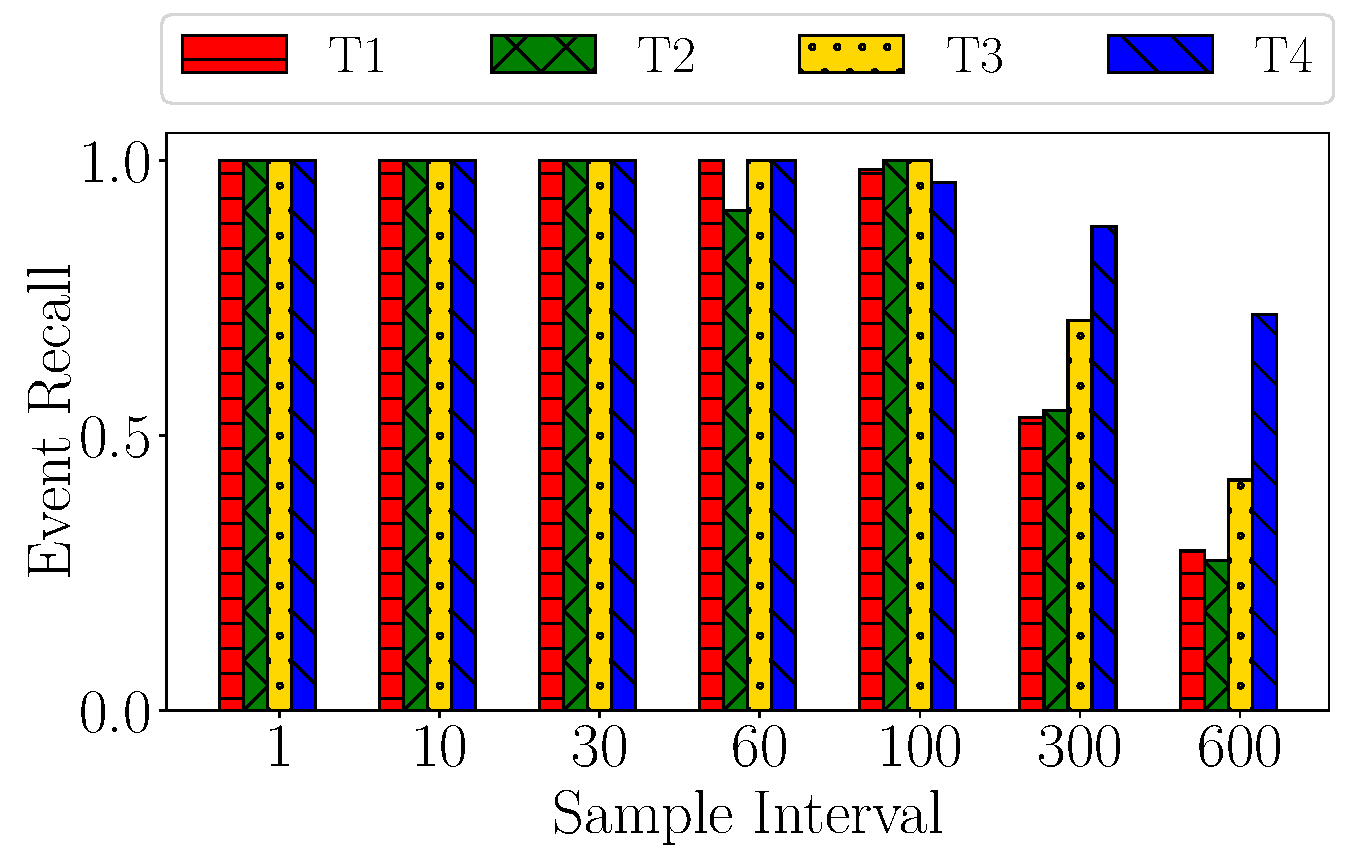
\includegraphics[width=\linewidth]{FIGS/fig-random-select-interval-recall-hatch.pdf}
\caption{Event Recall at Different Sampling Intervals}
\label{fig:sampling-only}
\end{figure}


  
\begin{figure}
    \centering
    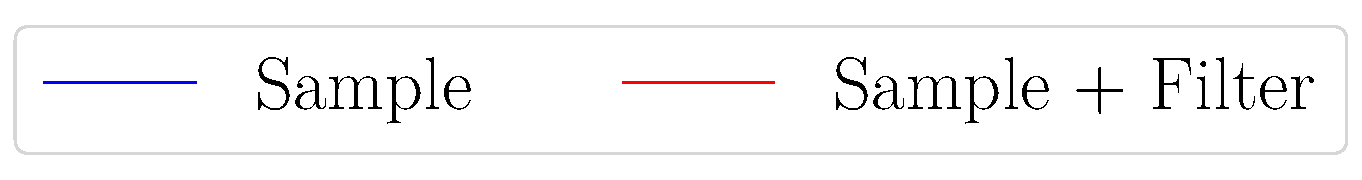
\includegraphics[width=0.7\linewidth]{FIGS/fig-recall-frame-aggregated-legend.pdf}
    \begin{subfigure}[T1]{
        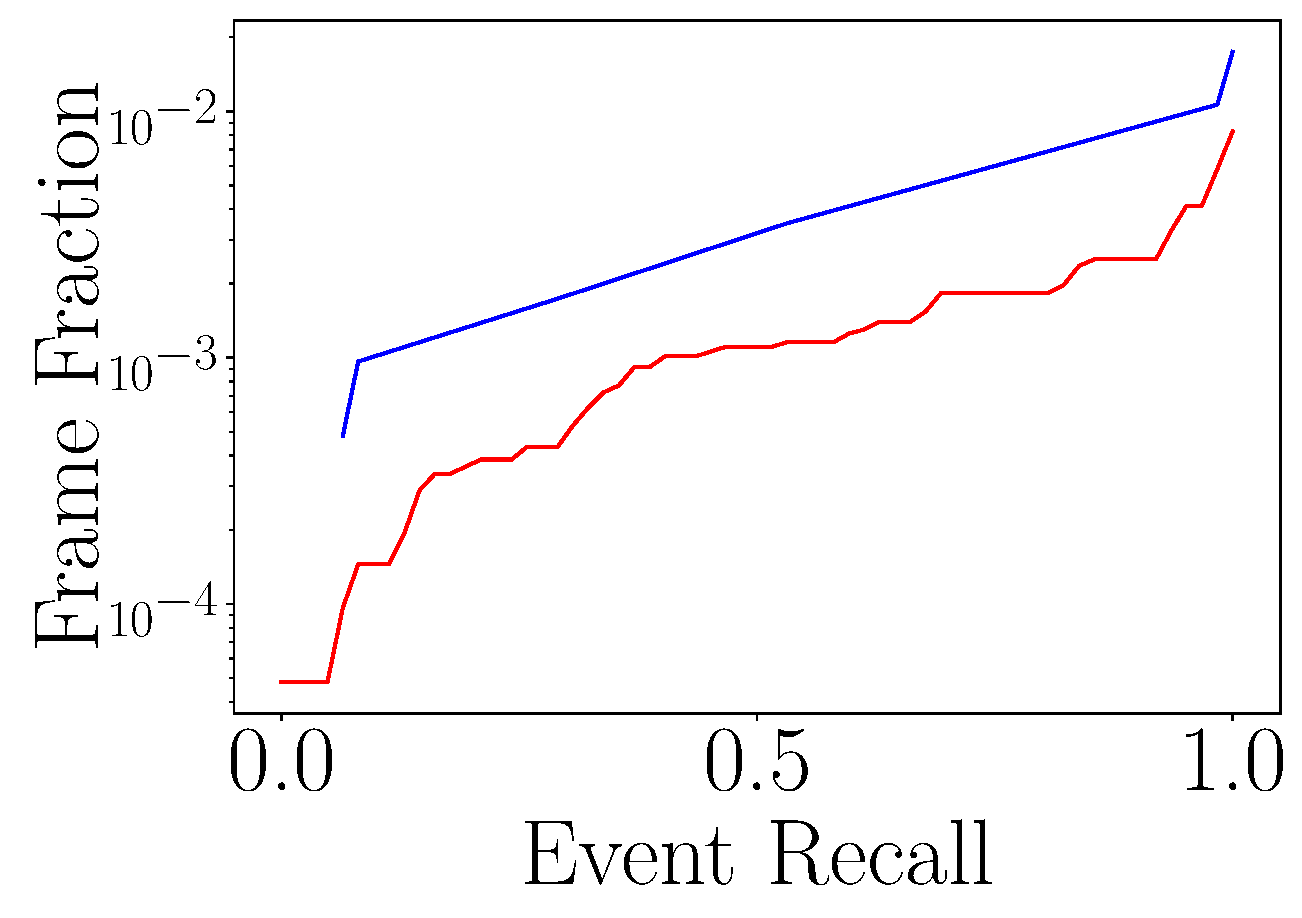
\includegraphics[trim={0.5cm 0.5cm 0 0},clip,width=0.47\linewidth]{FIGS/fig-random-select-and-filter-recall-frame-okutama-aggregated.pdf}}
    \end{subfigure}
    \begin{subfigure}[T2]{
      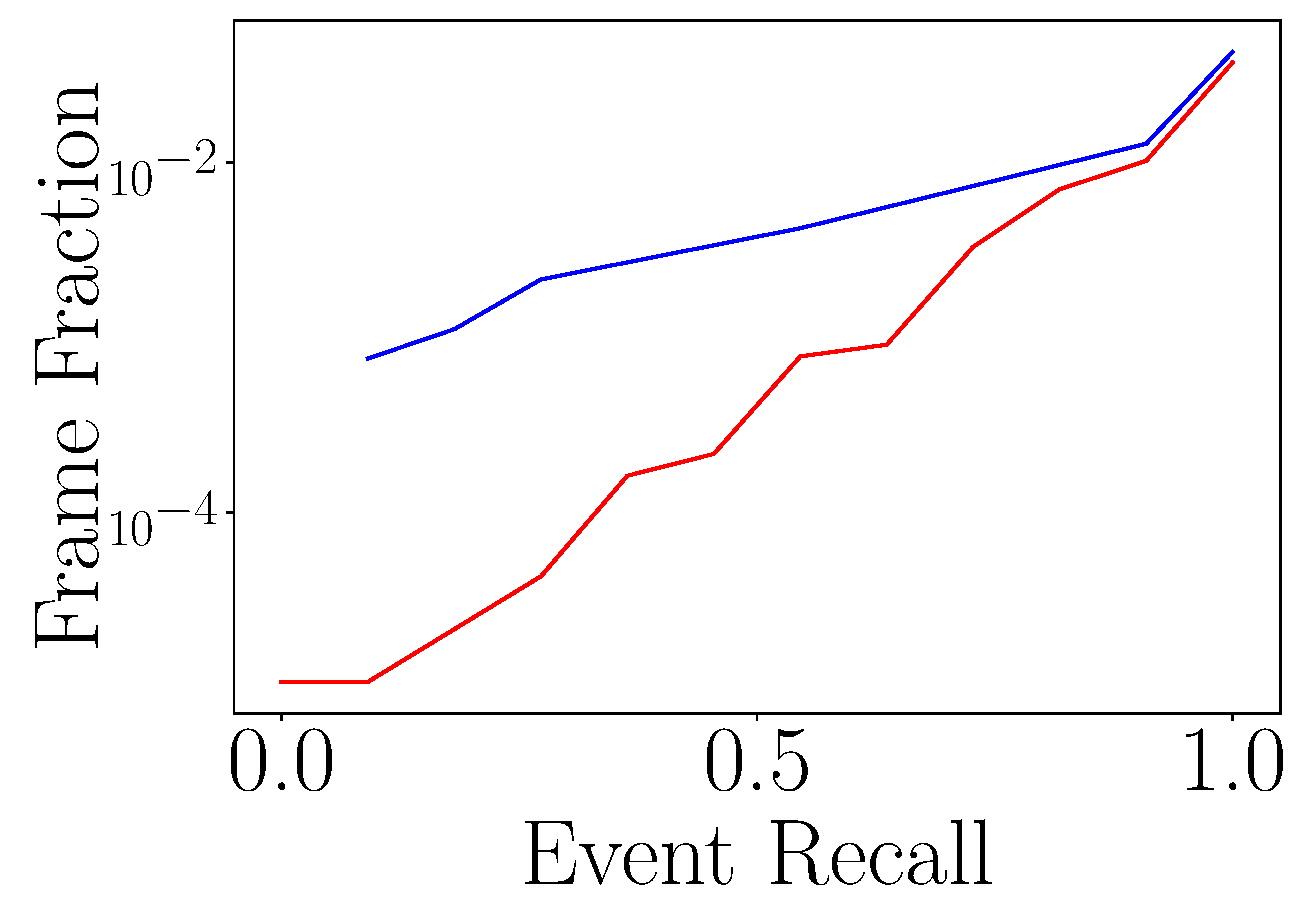
\includegraphics[trim={0.5cm 0.5cm 0 0},clip,width=0.47\linewidth]{FIGS/fig-random-select-and-filter-recall-frame-stanford-aggregated.pdf}}
    \end{subfigure}
    \begin{subfigure}[T3]{
      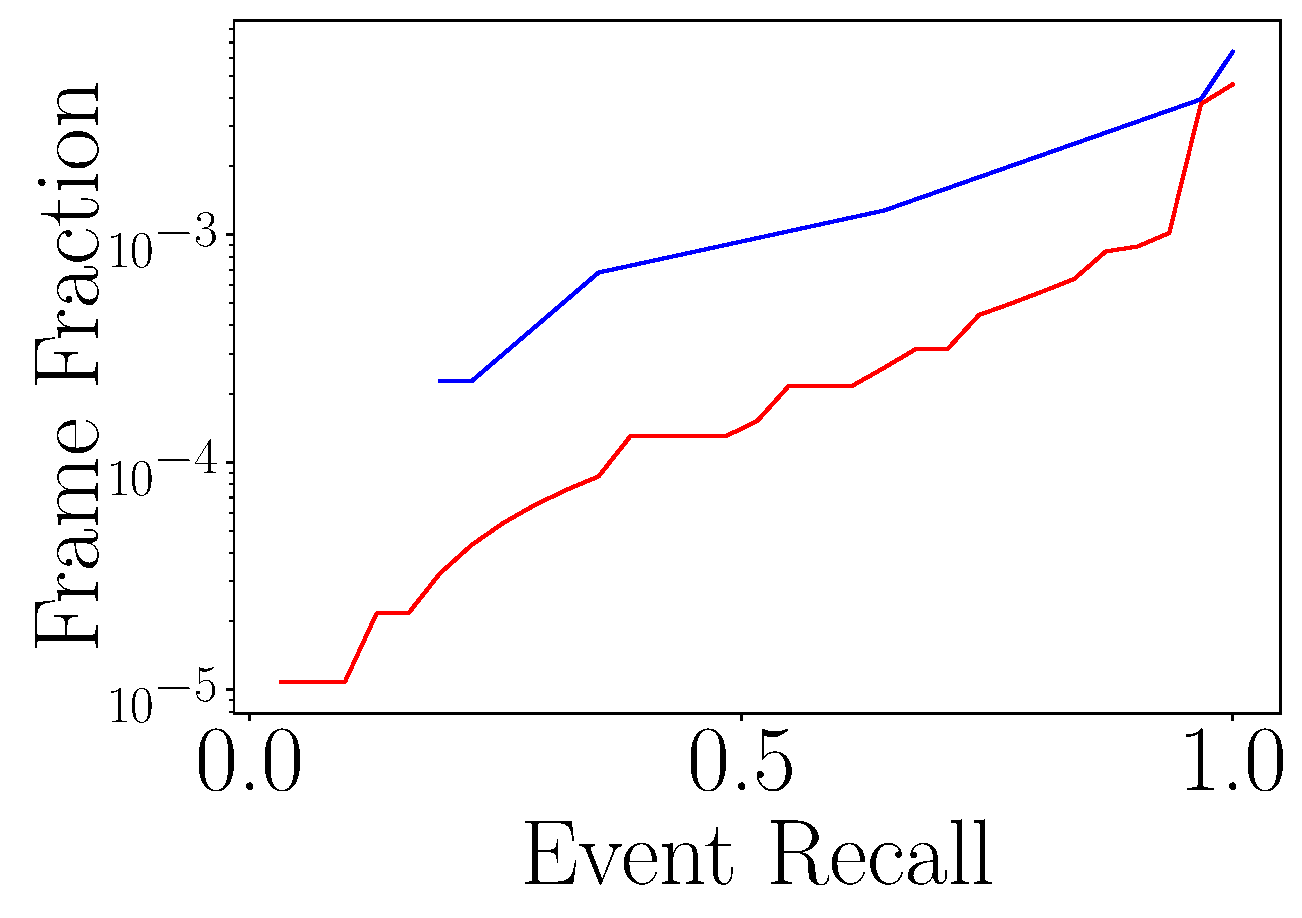
\includegraphics[trim={0.5cm 0.5cm 0 0},clip,width=0.47\linewidth]{FIGS/fig-random-select-and-filter-recall-frame-raft-aggregated.pdf}}
    \end{subfigure}
    \begin{subfigure}[T4]{
      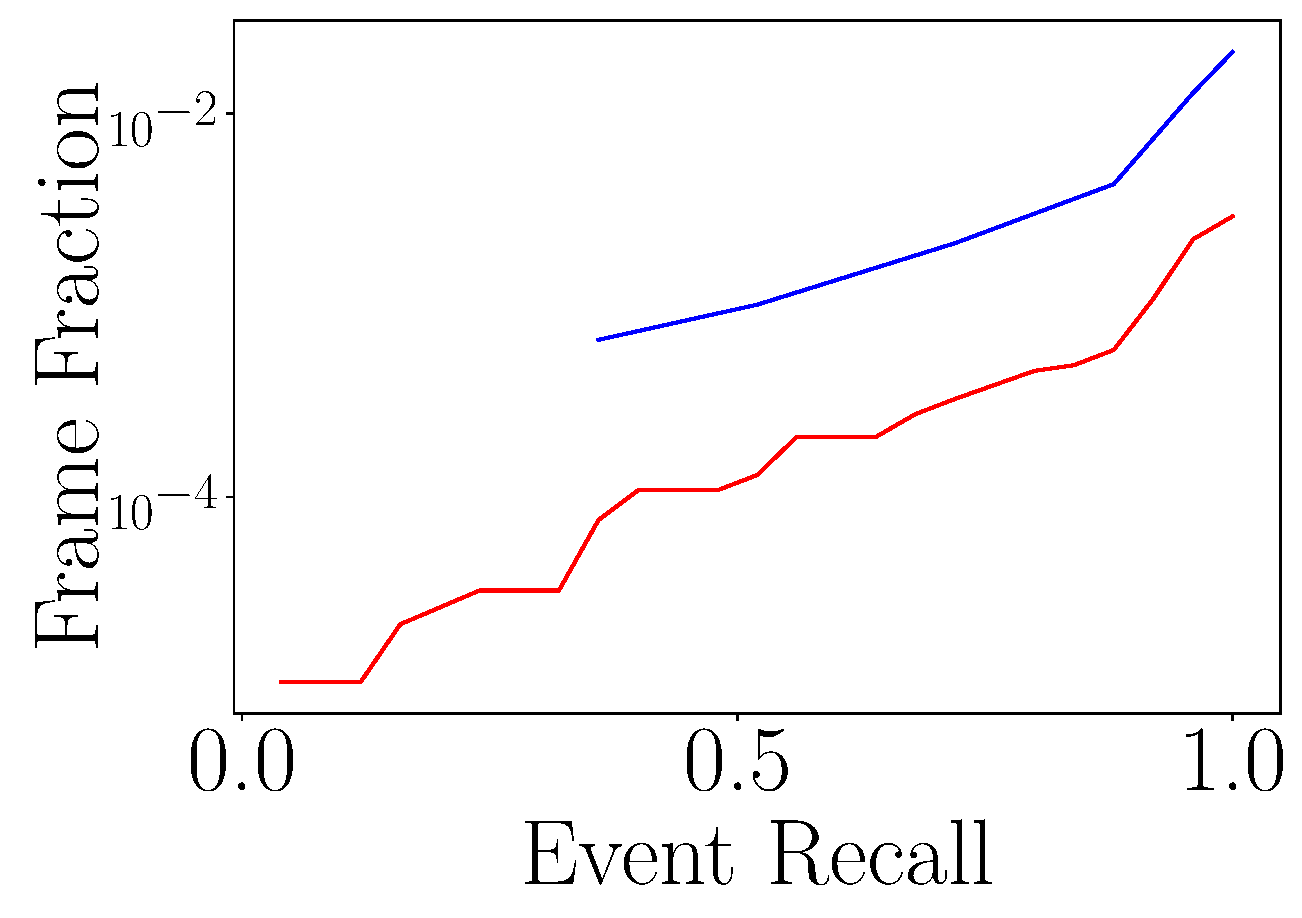
\includegraphics[trim={0.5cm 0.5cm 0 0},clip,width=0.47\linewidth]{FIGS/fig-random-select-and-filter-recall-frame-elephant-aggregated.pdf}}
    \end{subfigure}
    \vspace{-0.15in}
\caption{Sample with Early Discard. Note the log scale on y-axis.}
    \vspace{-0.15in}
\label{fig:sampling-discard}
\end{figure}

Given the relatively low precision of the weak detectors, a significant number 
of false positives are transmitted.  Furthermore, the occurrence of an object will
likely last through many frames, so true positives are also often redundant for 
simple detection tasks.  Both of these result in excessive
consumption of precious bandwidth.  
This suggests that simply restricting the number of transmitted
frames by sampling may help reduce bandwidth consumption.  

Figure~\ref{fig:sampling-only} shows the effects of 
sending a sample of frames from the drone, without any
content-based filtering.  Based on these results, we can reduce
the frames sent as little as one per second and still get
adequate recall at the cloudlet.  Note that this result is very
sensitive to the actual duration of the events in the videos.
For the detection tasks outlined here, most of the events (e.g.,
presences of a particular elephant) last for many seconds (100's
of frames), so such sparse sampling does not hurt recall.
However, if the events were of short duration, e.g., just a few
frames long, then this method would be less effective, as
sampling may lead to many missed events (false negatives).  

Can we use content-based filtering along with sampling to further
reduce bandwidth consumption?  Figure~\ref{fig:sampling-discard}
shows results when running early discard on a sample of the
frames. This shows that for the same recall, we can reduce the
bandwidth consumed by another factor of 5 on average over sampling alone.
This effective combination can reduce the average bandwidth
consumed for our test videos to just a few hundred kilobits
per second.  Furthermore, more processing time is available per
processed frame, allowing more sophisticated algorithms to be
employed, or to allow smaller tiles to be used, improving
accuracy of early discard.  

One case where sampling is not an effective solution is when all
frames containing an object need to be sent to the cloudlet for
some form of activity or behavior analysis from a complete video
sequence (as may be needed for task T5).  In this case, bandwidth
will not reduce much, as all frames in the event sequence must be
sent.  However, the processing time benefits of sampling may
still be exploited, provided all frames in a sample interval are
transmitted on a match.  


\subsection{Effects of Video Encoding}

\begin{figure}
\centering
\begin{tabular}{|p{1.5cm}|p{1.3cm}|p{1.3cm}|p{1.3cm}|}
\hline
JPEG Frame Sequence (MB)  & H264 High Quality (MB)       & H264 Medium Quality (MB) & H264 Low Quality (MB)\\
\hline
5823 & 3549  & 1833 & 147\\
\hline
\end{tabular}\\
\vspace{0.1in}
\begin{captiontext}
H264 high quality uses Constant Rate Factor (CRF) 23. Medium
uses CRF 28 and low uses 40~\cite{Merritt2007}.
\end{captiontext}
\caption{Test Dataset Size With Different Encoding Settings}
\label{fig:video-vs-images}
\end{figure}


One advantage of the {\xc DumbDrone} strategy is that since all
frames are transmitted, one can use a modern video encoding to
reduce transmission bandwidth.  With early discard, only a subset
of disparate frames are sent.  These will likely need to be
individually compressed images, rather than a video stream.  How
much does the switch from video to individual frames affect
bandwidth?  

In theory, this can be a significant impact. Video encoders leverage the
similarity between consecutive frames, and model motion to efficiently encode
the information across a set of frames. Image compression can only exploit
similarity within a frame, and cannot efficiently reduce number of bits needed
to encode redundant content across frames. To evaluate this difference, we start
with extracted JPEG frame sequences of our video data set. We encode the frame
sequence with different H.264 settings. Figure~\ref{fig:video-vs-images}
compares the size of frame sequences in JPEG and the encoded video file sizes.
We see only about 3x difference in the data size for the medium quality. We can
increase the compression (at the expense of quality) very easily, and are able
to reduce the video data rate by another order of magnitude before quality
degrades catastrophically.

However, this compression does affect analytics. Even at medium quality level,
visible compression artifacts, blurring, and motion distortions begin to appear.
Initial experiments analyzing compressed videos show that these distortions do
have a negative impact on accuracy of analytics. Using average precision
analysis, a standard method to evaluate accuracy, we see that the 
most accurate model (Faster-RCNN ResNet101) on low quality videos performs similarly
to the less accurate model (Faster-RCNN InceptionV2) on high quality
JPEG images. This negates the benefits of using the state-of-art models.

In this system, we pay a penalty of sending frames instead of a compressed low
quality video stream. This overhead (approximately 30x) is compensated by the
100x reduction in frames transmitted due to sampling with early discard. In
addition, the selective frame transmission preserves the accuracy of the
state-of-art detection techniques.

Finally, one other option is to treat the set of disparate frames as a sequence
and employ video encoding at high quality. This can ultimately eliminate the per
frame overhead while maintaining accuracy. However, this will require a complex setup with
both low-latency encoders and decoders, which can generate output data
corresponding to a frame as soon as input data is ingested, with no buffering,
and can wait arbitrarily long for additional frame data to arrive. 

For the experiments in the rest of the paper, we only account for the fraction
of frames transmitted, rather than the choice of specific encoding methods used
for those frames.



%-------------- LEAVE THIS AT THE END OF THIS FILE --------------------
\begin{comment}
% Satya: Save this old table because it has lots of details that 
% are not included in the smaller table that is in the paper
\begin{figure*}[]
\centering
\begin{tabular}{|p{2cm}|p{2cm}|p{2cm}|p{3cm}|p{3cm}|p{3cm}|}
\hline
Task                     & Task Description                                                                           & Dataset                & Dataset Description                                                                                                                & Train Videos                                                                                     & Test Videos                                                         \\ \hline
Human Detection 	& Detect human beings in daily life scene. Report any humans detected.			& 	UCF Aerial Action Dataset \href{http://crcv.ucf.edu/data/UCF_Aerial_Action.php}{link}				& A video dataset for aerial view of human actions. 4 videos, 107184 frames in total. 720x480 @ 30FPS. 			&  Select 2 videos with drone moving.  57430 frames.			& Select 2 videos with drone moving. 49754 frames.\\ \hline
Human Detection          & Detect human beings in a search and rescue scene. Report any humans detected.              & Okutama Action Dataset~\cite{Barekatain2017} 	& A video dataset for aerial view concurrent human action detection.  33 videos, 59842 frames in total. 3840x2160 @ 30FPS.           & Select 9 videos in which drones are actively moving, similar to search and rescue. 17763 frames. & Randomly select 3 videos in which drones are moving.  6014 frames.  \\ \hline
Human Activity Detection & Detect human activities such as waving hands                                               & Okutama Action Dataset & Same as above                                                                                                                      & Same as above                                                                                    & Same as above                                                       \\ \hline
Moving Car Detection     & Detect cars in a search and rescue scene that are moving. Report any moving cars detected. & Stanford Drone Dataset~\cite{Robicquet2016} & An aerial video dataset of cars and people navigating in a university campus. 60 videos, 522497 frames in total. $\sim$HD @ 30FPS. & Select 16 videos in which exists moving cars. 179992 frames.                                     & Randomly select 5 videos in which exists moving cars. 60249 frames. \\ \hline
Raft Detection           & Detect raft in a flooding scene                               & Collected 11 Youtube Videos \href{https://www.dropbox.com/sh/zksp1pzc1ix5hlw/AAB3HEhx-yLAJVR1Q3HnFpsWa?dl=0}{[Links]}       & Aerial-view videos with rafts. 11 videos. 54395 frames in total. $\sim$720P @ 30 FPS.                                                                                                    & 8 videos of rafting as training set. 43017 frames.                                      &  3 videos that resemble search and rescue scenarios. 11378 frames.                                               \\ \hline
Animal Detection         & Detect elephants in their natural habitat                     & Collected 11 Youtube Videos \href{https://www.dropbox.com/sh/3uly2qqwbzjasaa/AABiWSzPD_5uzmvCy3meqPKma?dl=0}{[Links]}      &  Aerial-view videos containing elephants in their natural habitat. 11 videos. 54203 frames in total. $\sim$720P @ 30FPS.                                                                         & Randomly selected 8 videos as training set. 39466 frames.                      & Randomly selected 3 videos as test set. 14737 frames.                \\ \hline
\end{tabular}
\caption{Task and Dataset}
\label{fig:task-and-dataset}
\end{figure*}
\end{comment}


\section{{\xc Just-in-time-Learning} S\lc{trategy} To Improve Early Discard}
\label{sec:jitl}

\subsection{Description}

Just-in-time-learning  (JITL) tunes the drone pipeline to the characteristics of
 the current mission in order to reduce transmitted false positives from the
 drone, and therefore reduce wasted bandwidth.  It is inspired by the cascade
 architecture from the computer vision community~\cite{Viola2001}, but is
 different in construction. A JITL filter is a cheap cascade filter that
 distinguishes between the EarlyDiscard DNN's \emph{true positives} (frames that
 are actually interesting) and \emph{false positives} (frames that are wrongly
 considered interesting).  Specifically, when a frame is reported as positive by
 EarlyDiscard, it is then passed through a JITL filter. If the JITL filter
 reports negative, the frame is regarded as a false positive and will not be
 sent. Ideally, all \emph{true positives} from EarlyDiscard are marked
 \emph{positive} by the JITL filter, and all \emph{false positives} from 
 EarlyDiscard are marked \emph{negative}.  Frames dropped by EarlyDiscard are
 not processed by the JITL filter, so this approach can only serve to improve
 precision, but not recall.


Periodically during a drone mission, a JITL filter is trained on the cloudlet
using the frames transmitted from the drone.  The frames received on the
cloudlet are predicted positive by the EarlyDiscard filter. The cloudlet, with
more processing power, is able to run more accurate DNNs to identify true
positives and false positives. Using this information, a small and lightweight
JITL filter is trained to distinguish true positives and false positives of
EarlyDiscard filters. These JITL filters are then pushed to the drone to run as
a cascade filter after the EarlyDiscard DNN.

True/false positive frames have high temporal locality throughout a drone
mission. The JITL filter is expected to pick up the features that confused the
EarlyDiscard DNN in the immediate past and improve the pipeline's accuracy in
the near future. These features are usually specific to the current flight, and
may be affected by terrain, shades, object colors, and particular shapes or
background textures.

JITL can be used with EarlyDiscard DNNs of different cutoff probabilities to
strike different trade-offs. In a bandwidth-favored setting, JITL can work with
an aggressively selective EarlyDiscard DNN to further reduce wasted bandwidth. In
a recall-favored setting, JITL can be used with a lower-cutoff DNN to preserve
recall.

In our implementation, we use a linear support vector machine
(SVM)~\cite{Friedman2001} as the JITL filter. Linear SVM has several advantages:
1) short training time in the order of seconds; 2) fast inference; 3) only
requires a few training examples; 3) small in size to transmit, usually on the
order of 50KB in our experiments. The input features to the JITL SVM filter are
the image features extracted by the EarlyDiscard DNN filter. In our case, since
we are using MobileNet as our EarlyDiscard filter, they are the 1024-dimensional
vector elements from the second last layer of MobileNet. This vector, also
called ``bottleneck values'' or ``transfer values'' captures high-level features
that represents the content of an image. Note that the availability of such
image feature vector is not tied to a particular image classification DNN nor
unique to MobileNet. Most image classification DNNs can be used as a feature
extractor in this way.

\subsection{Experimental Setup}
We used Jetson TX2 as our drone platform and evaluated the JITL strategy on four
tasks, T1 to T4. For the test videos in each task, we began with the
EarlyDiscard filter only and gradually trained and deployed JITL filters.
Specifically, every ten seconds, we trained an SVM using the frames transmitted
from the drone and the ground-truth labels for these frames. In a real
deployment, the frames would be marked as true positives or false positives by
an accurate DNN running on the cloudlet since ground-truth labels are not
available. In our experiments, we used ground-truth labels to control variables
and remove the effect of imperfect prediction of DNN models running on the
cloudlet. In addition, we used the true and false positives from all previous
intervals, not just the last ten seconds when training the SVM. The SVM, once
trained, is used as a cascade filter running after the EarlyDiscard filter on
the drone to predict whether the output of the EarlyDiscard filter is correct or
not. For a frame, if the EarlyDiscard filter predicts it to be interesting, but
the JITL filter predicts the EarlyDiscard filter is wrong, it would not be
transmitted to the cloudlet. In other words, following two criteria need to be
satisfied for a frame to be transmitted to the cloudlet: 1) EarlyDiscard filter
predicts it to be interesting 2) JITL filter predicts the EarlyDiscard filter is
correct on this frame.

\subsection{Results}

%\noindent{\textbf{Frame transmission and DNN cutoff}}
%In this experiment, we vary the cutoff probability of the DNN that runs before the JITL filter.
%For each dataset,
%we report the number of total transmitted frames and the number of transmitted true positive frames.
%For comparison, we also report the DNN's number when JITL is not activated.
%Figure \ref{fig:jitl-frame-cutoff} shows the results.
%In most cases, JITL helps reducing the total transmitted frames without significantly reducing true positives.
%T5 manifests the best example: JITL retains almost all true positives,
%while reducing total transmission observably.

%\begin{figure}
%\centering
%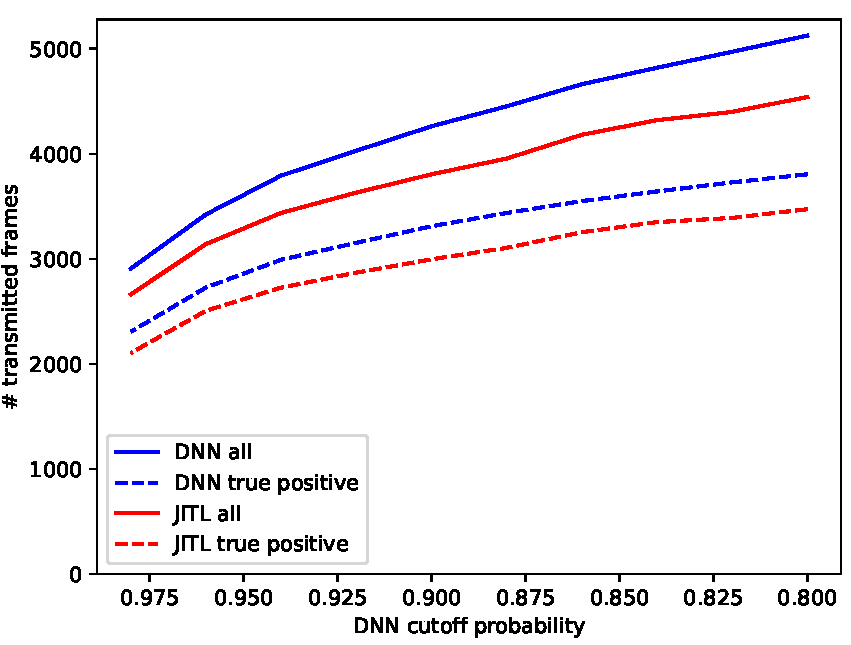
\includegraphics[width=0.6\linewidth]{FIGS/fig-jitl-okutama-frame.pdf}\\
%(a) T1\\[0.1in]
%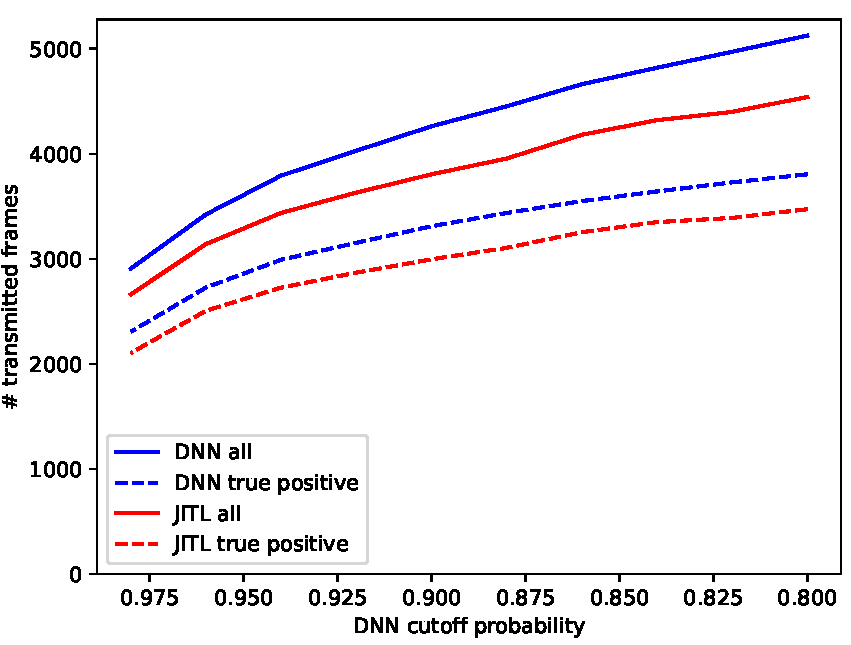
\includegraphics[width=0.6\linewidth]{FIGS/fig-jitl-okutama-frame.pdf}\\
%(b) T3\\[0.1in]
%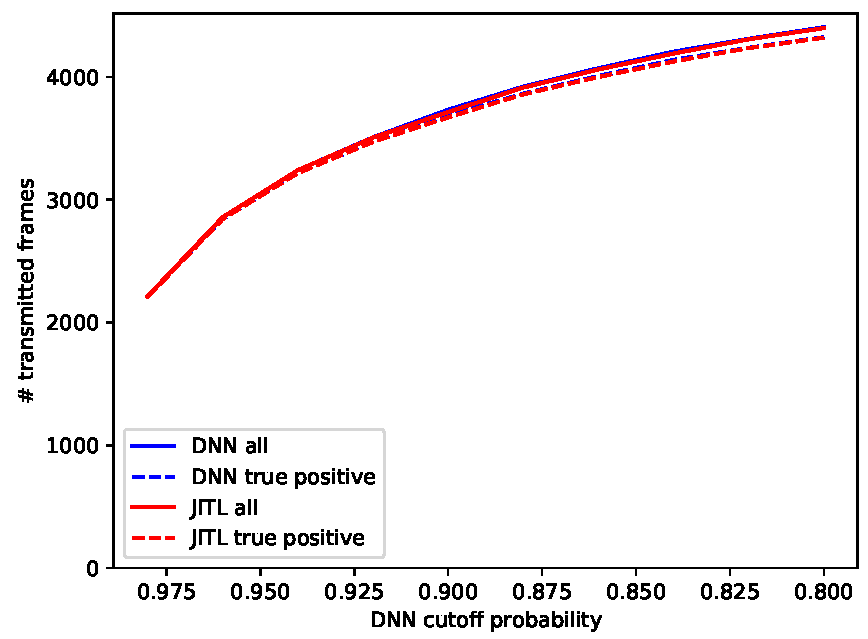
\includegraphics[width=0.6\linewidth]{FIGS/fig-jitl-raft-frame.pdf}\\
%(c) T4\\[0.1in]
%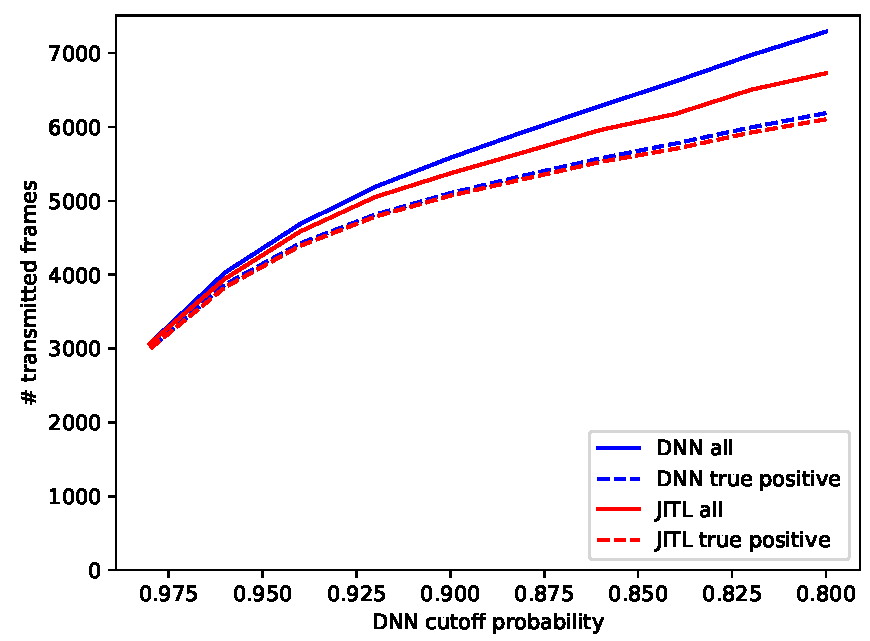
\includegraphics[width=0.6\linewidth]{FIGS/fig-jitl-elephant-frame.pdf}\\
%(d) T5\\[0.1in]
%\caption{Bandwidth vs. DNN Cutoff}
%\label{fig:jitl-frame-cutoff}
%\end{figure}


From our experiments, JITL is able to filter out more than 15\% of remaining
frames after EarlyDiscard without loss of event recall for three of four tasks.
Figure~\ref{fig:jitl-eventrecall} details the fraction of frames saved by JITL.
The x-axis presents event recall. Y-axis represents the fraction of total
frames. The blue region presents the achievable fraction of frames by
EarlyDiscard. The orange region shows the additional savings using JITL. For T1,
T3, and T4, at the highest event recall, JITL filters out more than 15\% of
remaining frames. This shows that JITL is effective at reducing the false
positives thus improving the precision of the drone filter. However,
occasionally, JITL predicts wrongly and removes true positives. For example, for
T2, JITL does not achieve a perfect event recall. This is due to shorter event
duration in T2, which results in fewer positive training examples to learn
from. Depending on tasks, getting enough positive training examples for JITL
could be difficult, especially when events are short or occurrences are few. To
overcome this problem in practice, techniques such as synthetic data
generation~\cite{Dwibedi2017} could be explored to synthesize true positives
from the background of the current flight.

\begin{figure}
    \centering
    
\includegraphics[trim={0 1.8cm 0 0},clip,width=0.7\linewidth]{FIGS/fig-jitl-legend.pdf}
    \hspace*{-0.3in}
    \begin{subfigure}[T1]{
        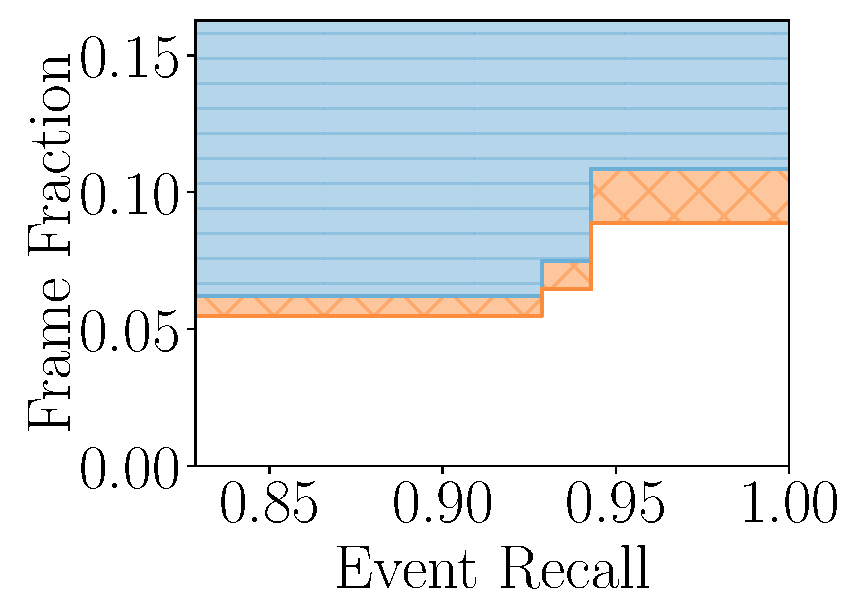
\includegraphics[width=0.5\linewidth]{FIGS/fig-jitl-okutama-eventrecall-step.pdf}}
    \end{subfigure}
    \begin{subfigure}[T2]{
        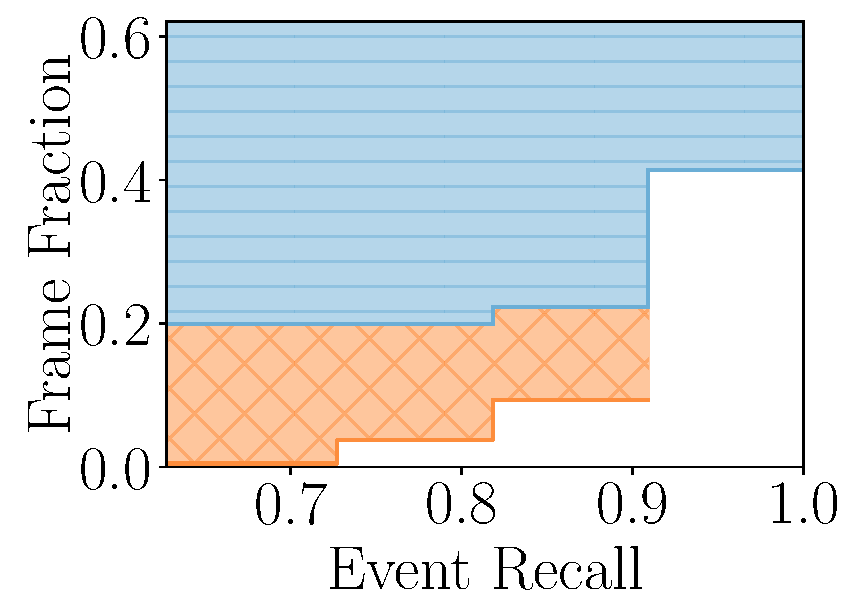
\includegraphics[width=0.5\linewidth]{FIGS/fig-jitl-stanford-eventrecall-step.pdf}}
    \end{subfigure}
    \hspace*{-0.3in}
    \begin{subfigure}[T3]{
        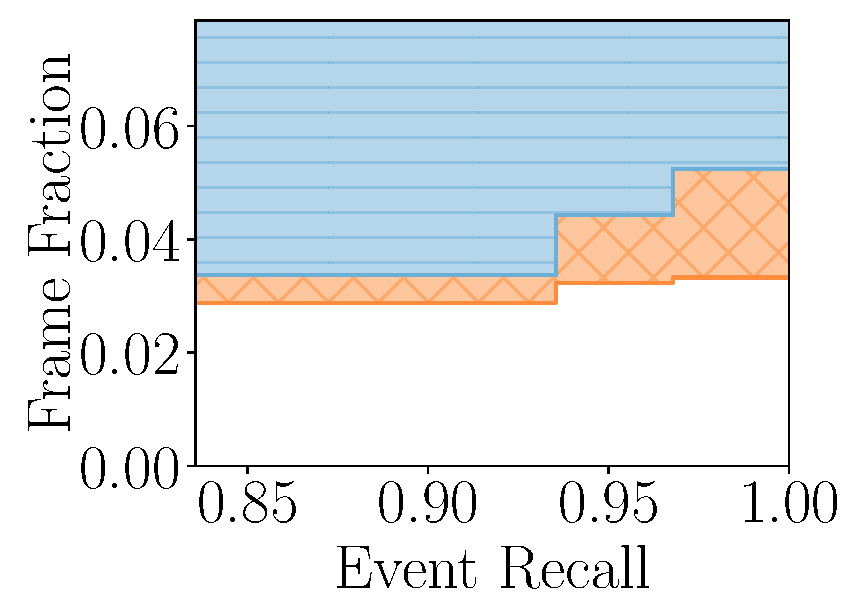
\includegraphics[width=0.5\linewidth]{FIGS/fig-jitl-raft-eventrecall-step.pdf}}
    \end{subfigure}
    \begin{subfigure}[T4]{
        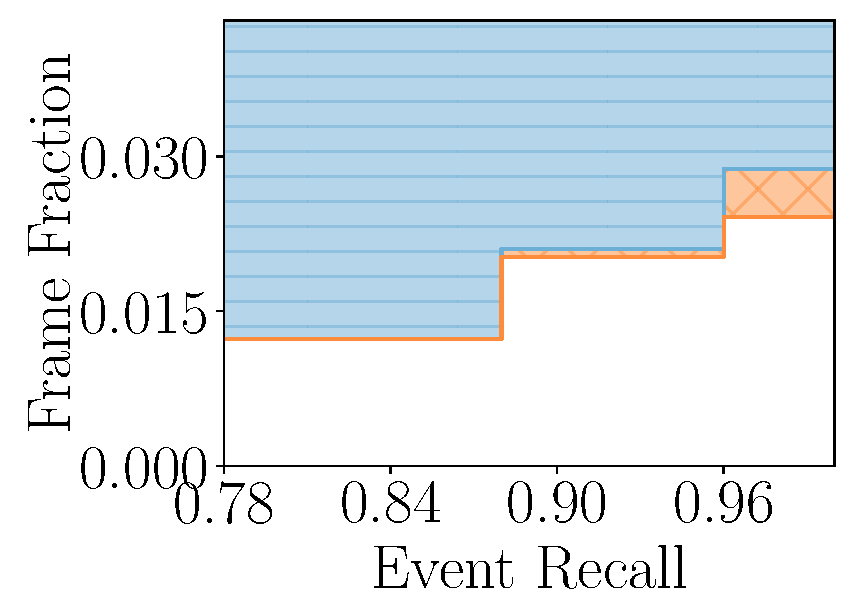
\includegraphics[width=0.5\linewidth]{FIGS/fig-jitl-elephant-eventrecall-step.pdf}}
    \end{subfigure}
\caption{JITL Fraction of Frames under Different Event Recall}
\label{fig:jitl-eventrecall}
\end{figure}

\section{Applying EARLYDISCARD and JITL to WCAs}
\label{bw:wca}

While the experiments in previous sections
(~\ref{sec:earlydiscard}~\ref{sec:jitl}) are performed in a drone video
analytics context, EarlyDiscard and JITL approaches can be applied more
generally to live video analytics offloading from Tier-3 devices to Tier-2 edge
data-centers. In this section, we use the LEGO
application~\cite{chen2018application} to showcase how to apply these bandwidth
saving approaches to WCAs.

\begin{figure}
\centering
\begin{minipage}[]{0.45\linewidth}
\centering
    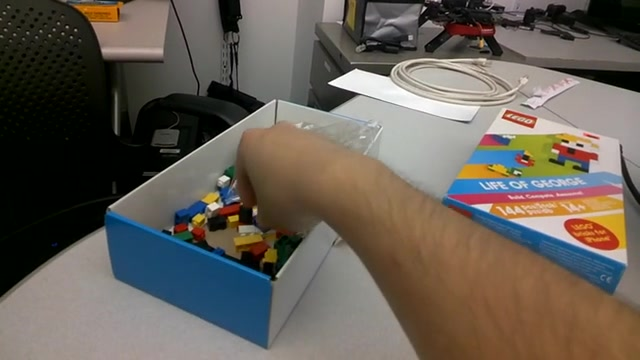
\includegraphics[width=\linewidth]{FIGS/lego-search}\\
{(a) Searching for Lego Blocks}
\end{minipage}
\begin{minipage}[]{0.45\linewidth}
\centering
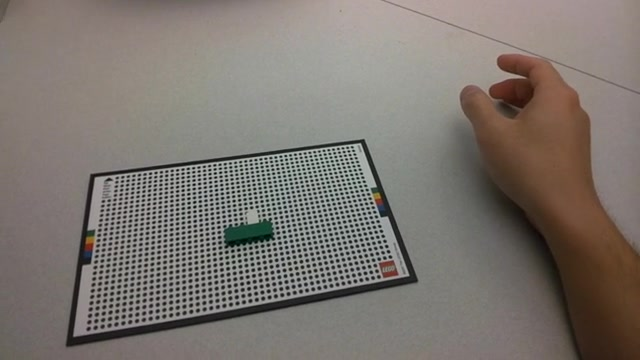
\includegraphics[width=\linewidth]{FIGS/lego-assembled}\\
{(b) Assmebling Lego Pieces}
\end{minipage}
\caption{Example Images from a Lego Assembly Video}
\label{fig:wca-lego-example-images}
\end{figure}

The LEGO wearable cognitive assistant helps a user put together a specific Lego
pattern by providing step-by-step audiovisual instructions. The application
works as follows. The assistant first prompts a user an animated image showing
the Lego block to use and asks the user to put it on the Lego board or assemble
it with previous pieces. Following the guidance, the user searches for the
particular Lego block, assemble it, and put the assembled piece on the Lego
board for the next instruction. Figure~\ref{fig:wca-lego-example-images} shows
the first-person view images captured from the wearable device during this
process. The assistant analyzes the assembled Lego piece on the Lego board by
identifying its shape and color using computer vision and provides the suitable
instruction.

\begin{figure}
\centering
\begin{minipage}[]{0.31\linewidth}
\centering
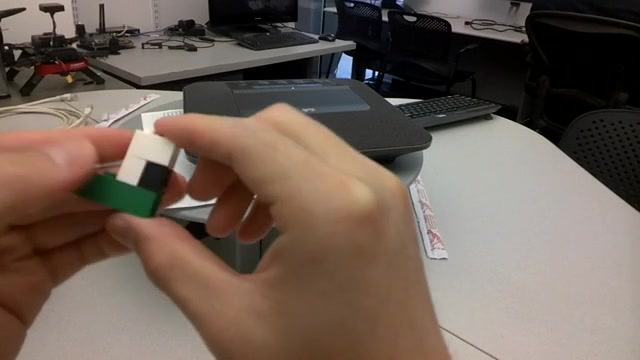
\includegraphics[width=\linewidth]{FIGS/lego-dataset-1}\\
\end{minipage}
\begin{minipage}[]{0.31\linewidth}
\centering
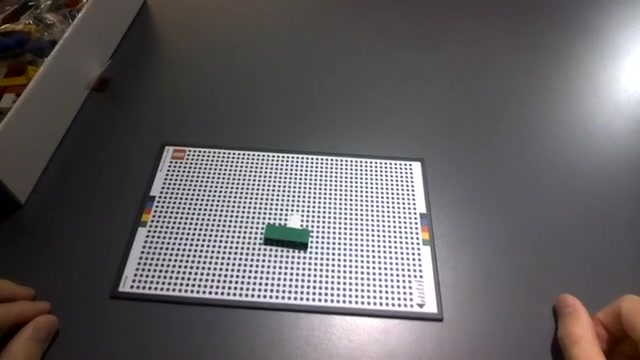
\includegraphics[width=\linewidth]{FIGS/lego-dataset-2}\\
\end{minipage}
\begin{minipage}[]{0.31\linewidth}
\centering
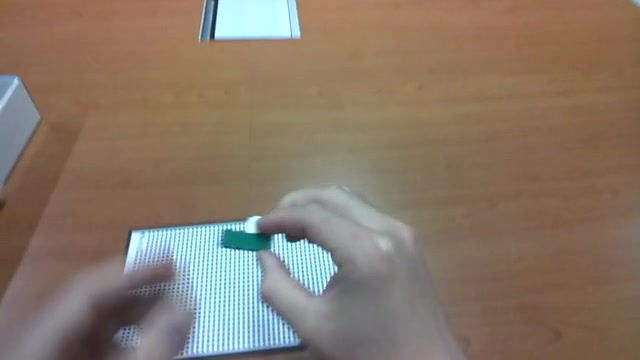
\includegraphics[width=\linewidth]{FIGS/lego-dataset-3}\\
\end{minipage}
\caption{Example Images from LEGO Dataset}
\label{fig:wca-lego-dataset}
\end{figure}

Intuitively, to the assistant, frames capturing the assembled piece on the Lego
board, (for example Figure~\ref{fig:wca-lego-example-images} (b)) are the
crucial frames to process, as they reflect the user's working progress.
Figure~\ref{fig:wca-lego-example-images} (a), on the other hand, is less
interesting as it does not contain information on user progress. If some cheap
processing on the wearable device could distinguish
(a) from (b), bandwidth consumption can be
reduced as we can discard Figure~\ref{fig:wca-lego-example-images} (b) early on
the wearable device without transmitting the frame to the cloudlet for processing.
This provides opportunities to apply EarlyDiscard and JITL.

We collect a LEGO dataset of twelve videos, in which users assemble Lego pieces
in three environments with different background, lighting, and viewpoints.
Figure~\ref{fig:wca-lego-dataset} shows example images from the dataset. We run
the LEGO WCA on these videos to get pseudo ground truth labels. Specifically,
for each frame, based on the outputs of the LEGO WCA vision processing, we
categorize the frame to be either ``interesting'' or ``not interesting''. A
frame is considered to be interesting if a LEGO board is found in the frame,
otherwise considered not interesting. 

\begin{figure}[h]
\centering
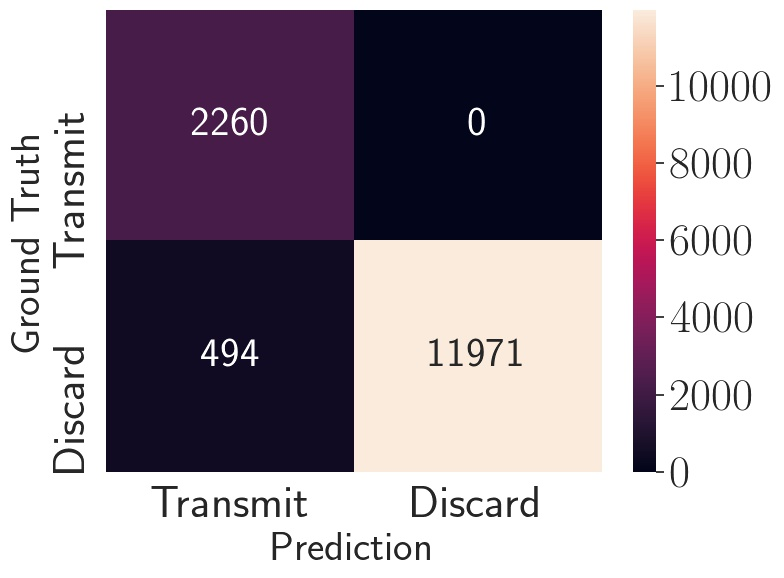
\includegraphics[width=.6\linewidth]{FIGS/earlydiscard-cm}\\
\caption{EarlyDiscard Filter Confusion Matrix}
\label{fig:wca-early-discard}
\end{figure}

We use this dataset to finetune a MobileNet DNN in order to automatically
distinguish interesting frames from the boring ones for EarlyDiscard. For each
of the three environments, we randomly select two videos for training, one video
for validation, and one video for testing. We randomly sample 2000 interesting
images and 2000 boring images from the six training videos as the training
data. Similarly, we random sample 200 interesting images and 200 boring images
from the three validation videos as the validation data. We implement
MobileNet transfer learning using the PyTorch
framework~\cite{paszke2019pytorch}. We train the model for 20 epochs and
select the model weights that give the highest accuracy on the validation set as
the model for inference.

Our test sets have in total 14725 frames. Figure~\ref{fig:wca-early-discard}
shows the confusion matrix of our trained EarlyDiscard classifier. X-axis
represents the predicted results: ``Transmit'' means the frame is predicted to
be interesting and should be transmitted to cloudlet for processing while
``Discard'' means the frame is predicted to be boring and should not be
transmitted. Similarly, Y-axis represents the ground truth results. As we can
see, the classifier correctly predicts 2260 out of 14725 frames to be
interesting and correctly suppresses 11971 frames. With EarlyDiscard in place,
only 19\% of all the frames are transmitted. Meanwhile, the false negative is 0
frame, meaning no ``interesting'' frame is wrongly discarded. This is the result
of biasing the classifier towards recall instead of precision. 

\begin{figure}
\centering
\begin{minipage}[b]{.45\linewidth}
\centering
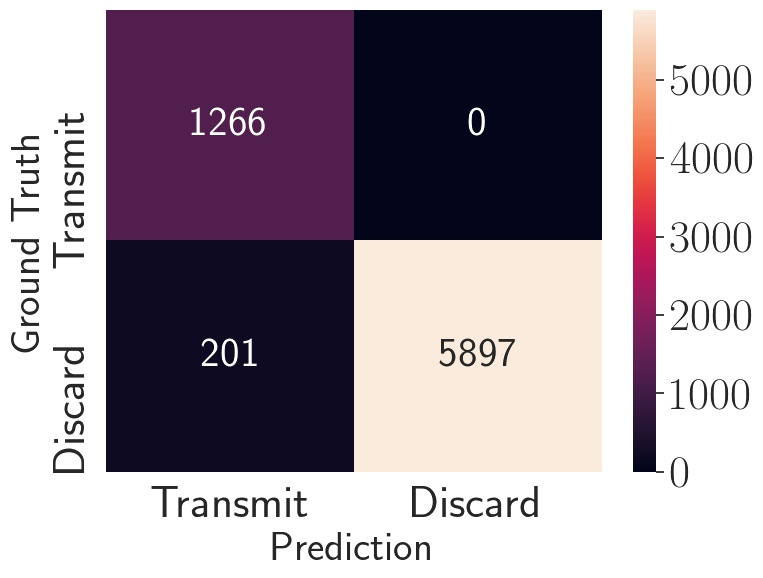
\includegraphics[width=\linewidth]{FIGS/jitl-earlydiscard-cm}\\
{(a) EarlyDiscard}
\end{minipage}
\begin{minipage}[b]{.45\linewidth}
\centering
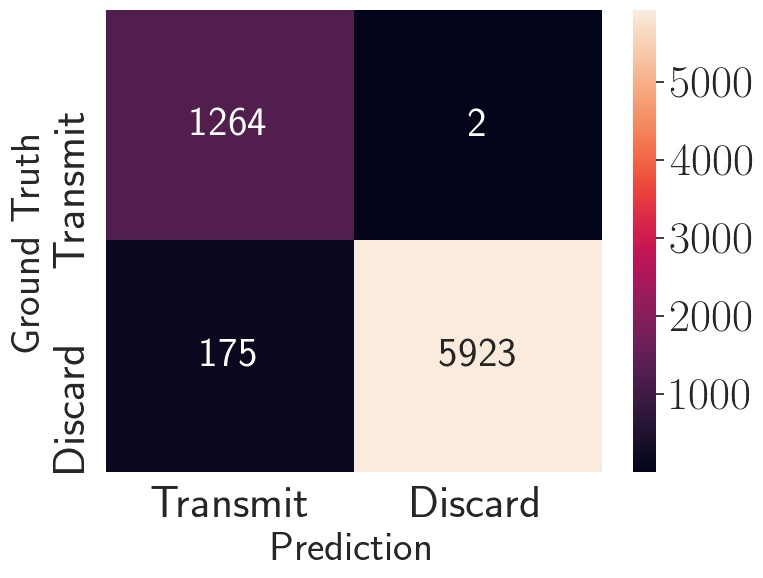
\includegraphics[width=\linewidth]{FIGS/jitl-combined-cm}\\
{(b) EarlyDiscard + JITL}
\end{minipage}
\caption{JITL Confusion Matrix}
\label{fig:wca-jitl}
\end{figure}

Among all the frames that are transmitted, 18\% of them are false positives.
These 494 false positives suggest that there are room to improve using JITL. For
each of the test videos, we use the first half of the video as training examples
for JITL to train a SVM that produces a confidence score for EarlyDiscard
prediction. Figure~\ref{fig:wca-jitl} compares the confusion matrix of using
EarlyDiscard alone with EarlyDiscard + JITL. As we can see, JITL reduces 13\% of
the false positives at the cost of 2 false negatives. Note that these 2 false
negative frames do not result in missing instructions as adjacent interesting
frames are still transmitted. 

% To reduce bandwidth consumption with EarlyDiscard and JITL, we first need to
% identify what frames should be considered interesting.

% the cheap computer vision processing that can identify ``interesting'' frames on
% Tier-3 devices. Figure~\ref{fig:wca-lego-example-images} provides intuitions on how to
% apply EarlyDiscard and JITL to the Lego application

\section{Discussion}
\label{bw:discussion}

The EarlyDiscard technique employs on-board filters to select interesting
frames and suppress the transmission of mundane frames to save bandwidth. In
particular, cheap yet effective DNN filters are trained offline to fully
leverage the large quantity of training data and the high learning capacities of
DNNs. Building on top of EarlyDiscard, JITL adapts an EarlyDiscard filter to a
specific mission environment online. Throughout a flight, JITL continuously
evaluates the EarlyDiscard filter and reduces the number of false positives by
predicting whether an EaryDiscard decision is made correctly. These two
techniques together reduce the total number of unnecessary frames transmitted.
In addition, some missions need consecutive frames instead of individual images
to do tasks such as activity recognition. Reachback compensates for these
scenarios when EarlyDiscard and JITL are deployed. Once the cloudlet identifies
an interesting frame from the data sent back by the drone, nearby frames are
pulled from storage on the drone. Furthermore, either an algorithm or a person
in the loop can determine when to trigger reachback. Besides reachback, the
person in the loop may also identify unique characteristics to create more
effective context-aware filters to increase accuracy and reduce on-board
computation.

\section{Related Work}
\label{bw:relatedwork}

The work presented in this paper is disjoint from these previous drone-centric
research efforts. Our focus is on reducing wireless transmission for live video
from autonomous drones in use cases such as search and rescue, surveillance, and
wildlife conservation. Wang et al.~\cite{Wang2017networked} shares our concern
for wireless bandwidth, but focuses on coordinating a network of drones to
capture and broadcast live sport event. In addition, Wang et
al~\cite{Wang2016skyeyes} explored adaptive video streaming with drones using
content-based compression and video rate adaptation. While we share their
inspiration, our work leverages characteristics of DNNs and explore human-in-the
loop to enable mission-specific optimization strategies including reachback and
context-awareness.

Much previous work on static camera networks and video analytics systems
explored efficient use of compute and network resources at scale. Zhang et
al.~\cite{zhang2017live} studied resource-quality trade-off under result latency
constraints in video analytics systems. Kang et al.~\cite{kang2017noscope} worked
on optimizing DNN queries over videos at scale. While they focus on supporting a
large number of computer vision workload, our work optimizes for the first hop
wireless bandwidth. In addition, Zhang et al.~\cite{zhang2015design} designed a
wireless distributed surveillance system that supports a large geographical area
through frame selection and content-aware traffic scheduling. In contrast, our
work uses drone moving cameras. We explore techniques that tolerate changing
scenes in video feeds and strategies that can leverage the human operator.

Some previous work on computer vision in mobile settings has relevance to
aspects of our system design.  Chen et al.~\cite{chen2015glimpse} explore how
continuous real-time object recognition can be done on mobile devices. They meet
their design goals by combining expensive object detection with computationally
cheap object tracking.  Although we do not use object tracking in our work, we
share the resource concerns that motivate that work.  Naderiparizi et
al.~\cite{naderiparizi2017glimpse} describe a programmable early-discard camera
architecture for continuous mobile vision.  Our work shares their emphasis on
early discard, but differs in all other aspects.  In fact, our work can be
viewed as complementing that work: their programmable early-discard camera would
be an excellent choice for our drones. Lastly, Hu et al~\cite{Hu2015} have
investigated the approach of using lightweight computation on a mobile device to
improve the overall bandwidth efficiency of a computer vision pipeline that
offloads computation to the edge.  We share their concern for wireless
bandwidth, and their use of early discard using inexpensive algorithms on the
mobile device.  However, their work is not in a drone setting and has no
counterpart to just-in-time learning, reachback, or context-aware discard
described in our work.
